%%==================================================
%% chapter02.tex for SJTU Master Thesis
%% based on CASthesis
%% modified by wei.jianwen@gmail.com
%% version: 0.3a
%% Encoding: UTF-8
%% last update: Dec 5th, 2010
%%==================================================

% \bibliographystyle{sjtu2} %[此处用于每章都生产参考文献]

\chapter{信道状态采样与估计}
\label{chap:phy}

安全始终是高速铁路发展过程中的首要目标,而GSM-R网络则是保证高铁系统安全性的重要环节,因此有必要对GSM-R网络进行在线实时测试,在确保GSM-R网络正常通信的基础之上,保证整个高铁系统的稳定运行。但是由于高铁系统具有较为特殊的无线传播环境,传统的信号强度测试算法无法直接应用于GSM-R网络测试中,例如高铁线路周围地形复杂多变以及列车处于高速运行状态,这就要求GSM-R网络信号强度测试算法必须具有实时高效的特点,以适应高速铁路的特殊要求。

\section{问题描述}
\label{sec:problem2}

\begin{figure}[!htp]
\centering
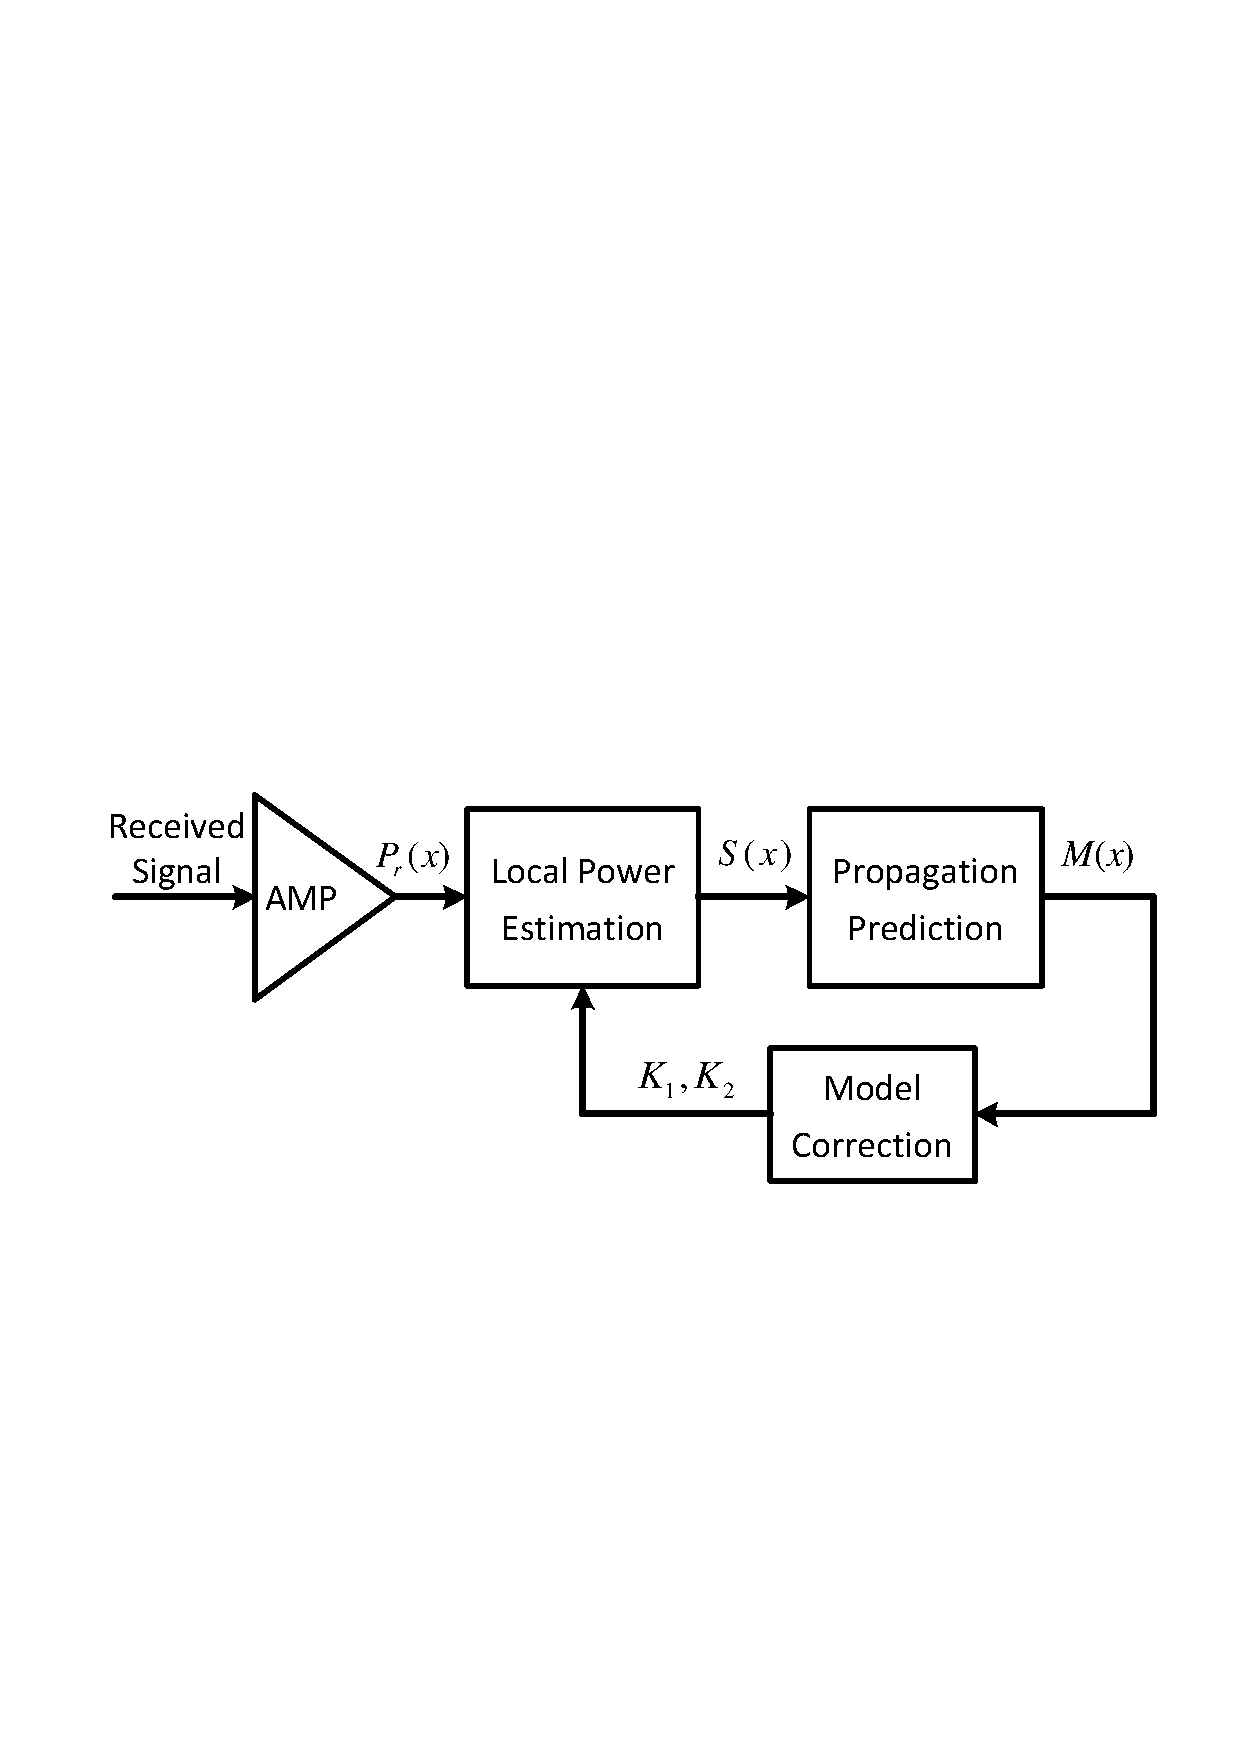
\includegraphics[width=4in]{chap2/measurement.pdf}
\bicaption[fig:measurement]{接收信号强度测试过程}{接收信号强度测试过程}{Fig}{Basic Procedures of Radio Propagation Measurement}
\end{figure}

无线网络接收信号强度测试过程如图 \ref{fig:measurement} 所示,测试系统通过包络检测得到接收信号强度,然后通过信号动态采样算法,得到当前阴影衰落与多径衰落信息,一方面用来对网络通信状态进行评估,另一方面作为网络越区切换的判断依据。同时根据采样数据进行无线传播预测,对网络的覆盖情况进行评估,最后对估计算法与预测模型进行参数修正。

\subsection{现有工作}
\label{sec:current3}

\begin{figure}[!htp]
\centering
    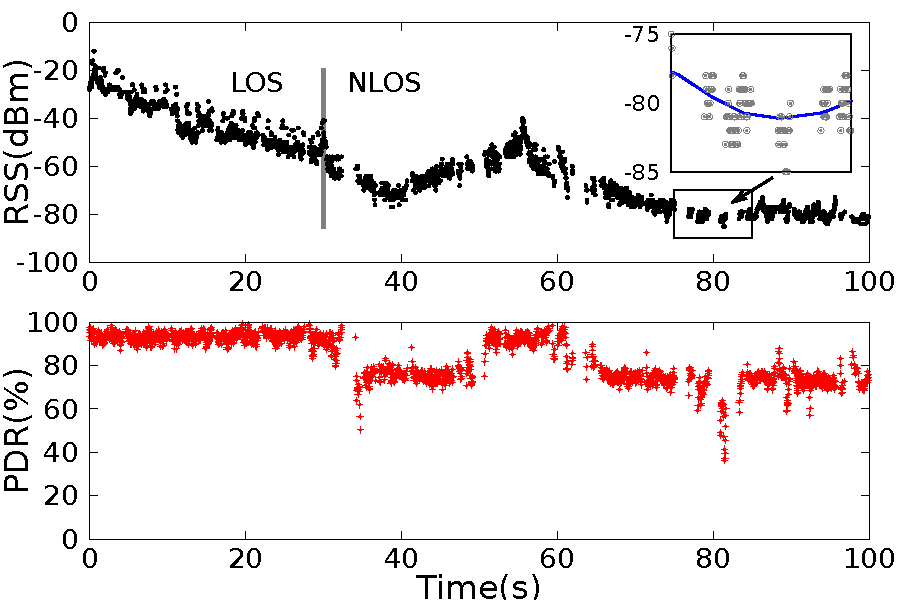
\includegraphics[width=5in]{chap2/time.pdf}
\bicaption[fig:timevary]{移动无线网络时变特性}{移动无线网络时变特性}{Fig}{Time varying of RSS in mobile wireless networks}
\end{figure}

移动无线网络信号强度测试的一个基本问题是本地均值的可靠估计,即如何确定合适的采样参数以准确地获取当前信号强度,同时在测试精度与开销之间实现合理平衡。移动无线网络接收信号强度通过特定统计区间内一定数量的采样点数的算术平均获得,因此采样频率决定了信号强度的测试精度与开销,因此需要根据无线传播环境的变化对信号的采样频率进行实时调整,对于GSM-R网络而言合理有效的采样精度与开销的平衡尤为重要。

如图 \ref{fig:timevary} 所示,移动无线网络接收信号强度具有明显的时变特性,其中包括大尺度衰落和小尺度衰落,如果信号采样的统计区间过长或采样频率过低,系统将无法对小尺度衰落作出合理评估,从而难以保证可靠的数据传输;相反,如果统计区间过段或采样频率过高,大尺度衰落和小尺度衰落难以有效区分,从而导致网络状态的不稳定,例如接收信号强度在切换门限附近波动造成的乒乓切换效应。

William C. Y. Lee在1985年最先提出移动网络信号强度采样算法,即Lee氏采样算法 \cite{lee1985estimate},该算法以移动网络无线传播传播模型为基础,在无线传播环境服从瑞利衰落的假设条件下,推导出信号强度的本地均值测量中的统计区间长度与采样点数。Mark D. Austin在其蜂窝网络的切换算法中对莱斯衰落条件下的采样算法进行了推导 \cite{Austin1994},得到统计区间与采样点数的近似解,但是该算法过程复杂且计算量较大。David de la Vega在2009年提出通用Lee氏采样算法 \cite{Vega2009},在不需要知道多径衰落具体分布的条件下,利用实测采样信号进行估计,得到实际网络环境所需要的统计区间与采样点数。由于高速铁路无线环境的复杂性及其对安全性的特殊要求,以上的本地均值估计算法难以在较低的测试开销条件下实现可靠的测试精度,不符合高铁环境实时测试的要求,因此无法直接应用于GSM-R网络中。

\subsection{存在问题}
\label{sec:prob3}

\begin{itemize}
  \item \textbf{高速移动特性}
  GSM-R网络处于高速运行状态,相同情况下需要对接收信号强度进行更为频繁的采样,对于900MMHz的通信频率,Lee氏采样算法的采样间隔为36cm,工程应用时一般选择4cm,在300km/h的运行速度下需要采样时间间隔达到432/48ms,而如此高的采样频率应用到在线测试时会严重影响到网络的正常通信。因此需要利用信道状态的时空相关性降低测试开销,同时满足高速移动条件下的测试精度。
  \item \textbf{无线传播环境}
  GSM-R网络一般存在直射路径,因此应当采用莱斯信道对GSM-R网络的无线传播环境进行刻画。现有工作主要针对瑞利衰落信道,直接应用与GSM-R 网络中时无法获得应有的测试精度。同时瑞利衰落情况下给出的采样参数为固定值,不能适应高速铁路复杂的无线传播环境。因此需要对莱斯衰落信道下的信道状态采样与估计进行分析,以适应高速铁路的无线传播环境。
\end{itemize}

\begin{figure}[!htp]
\centering
    \label{}
    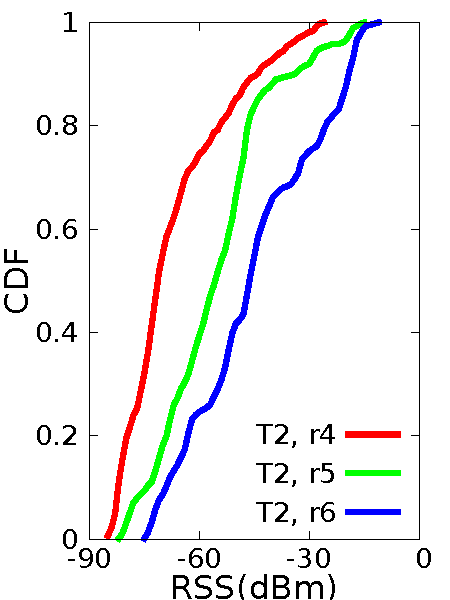
\includegraphics[width=2in]{chap2/cdfrss.pdf}
\bicaption[fig:cdfrss]{移动无线网络位置差异性}{移动无线网络位置差异性}{Fig}{Location differences of RSS in mobile wireless networks}
\end{figure}


\section{无线传播模型}
\label{sec:channelmodel}

由于高速铁路沿线地形复杂多变,一条线路通常会经过山地、平原、隧道和高架等地形,如图 \ref{fig:terrain} 所示,从而造成GSM-R网络无线传播环境的复杂性。同时图 \ref{fig:terrain} 中可以看出,高速铁路无线传播环境大多较为平坦,同时为了尽量保证GSM-R网络的可靠性,基站位置通常距离高铁线路很近,而且小区半径一般设置为3-6km,从而造成移动终端与基站之间一般存在直射LOS路径,因此GSM-R网络的无线传播应该刻画为莱斯衰落。

\begin{figure}[!htp]
\centering
\subfigure[高架]{
    \label{fig:viaduct}
    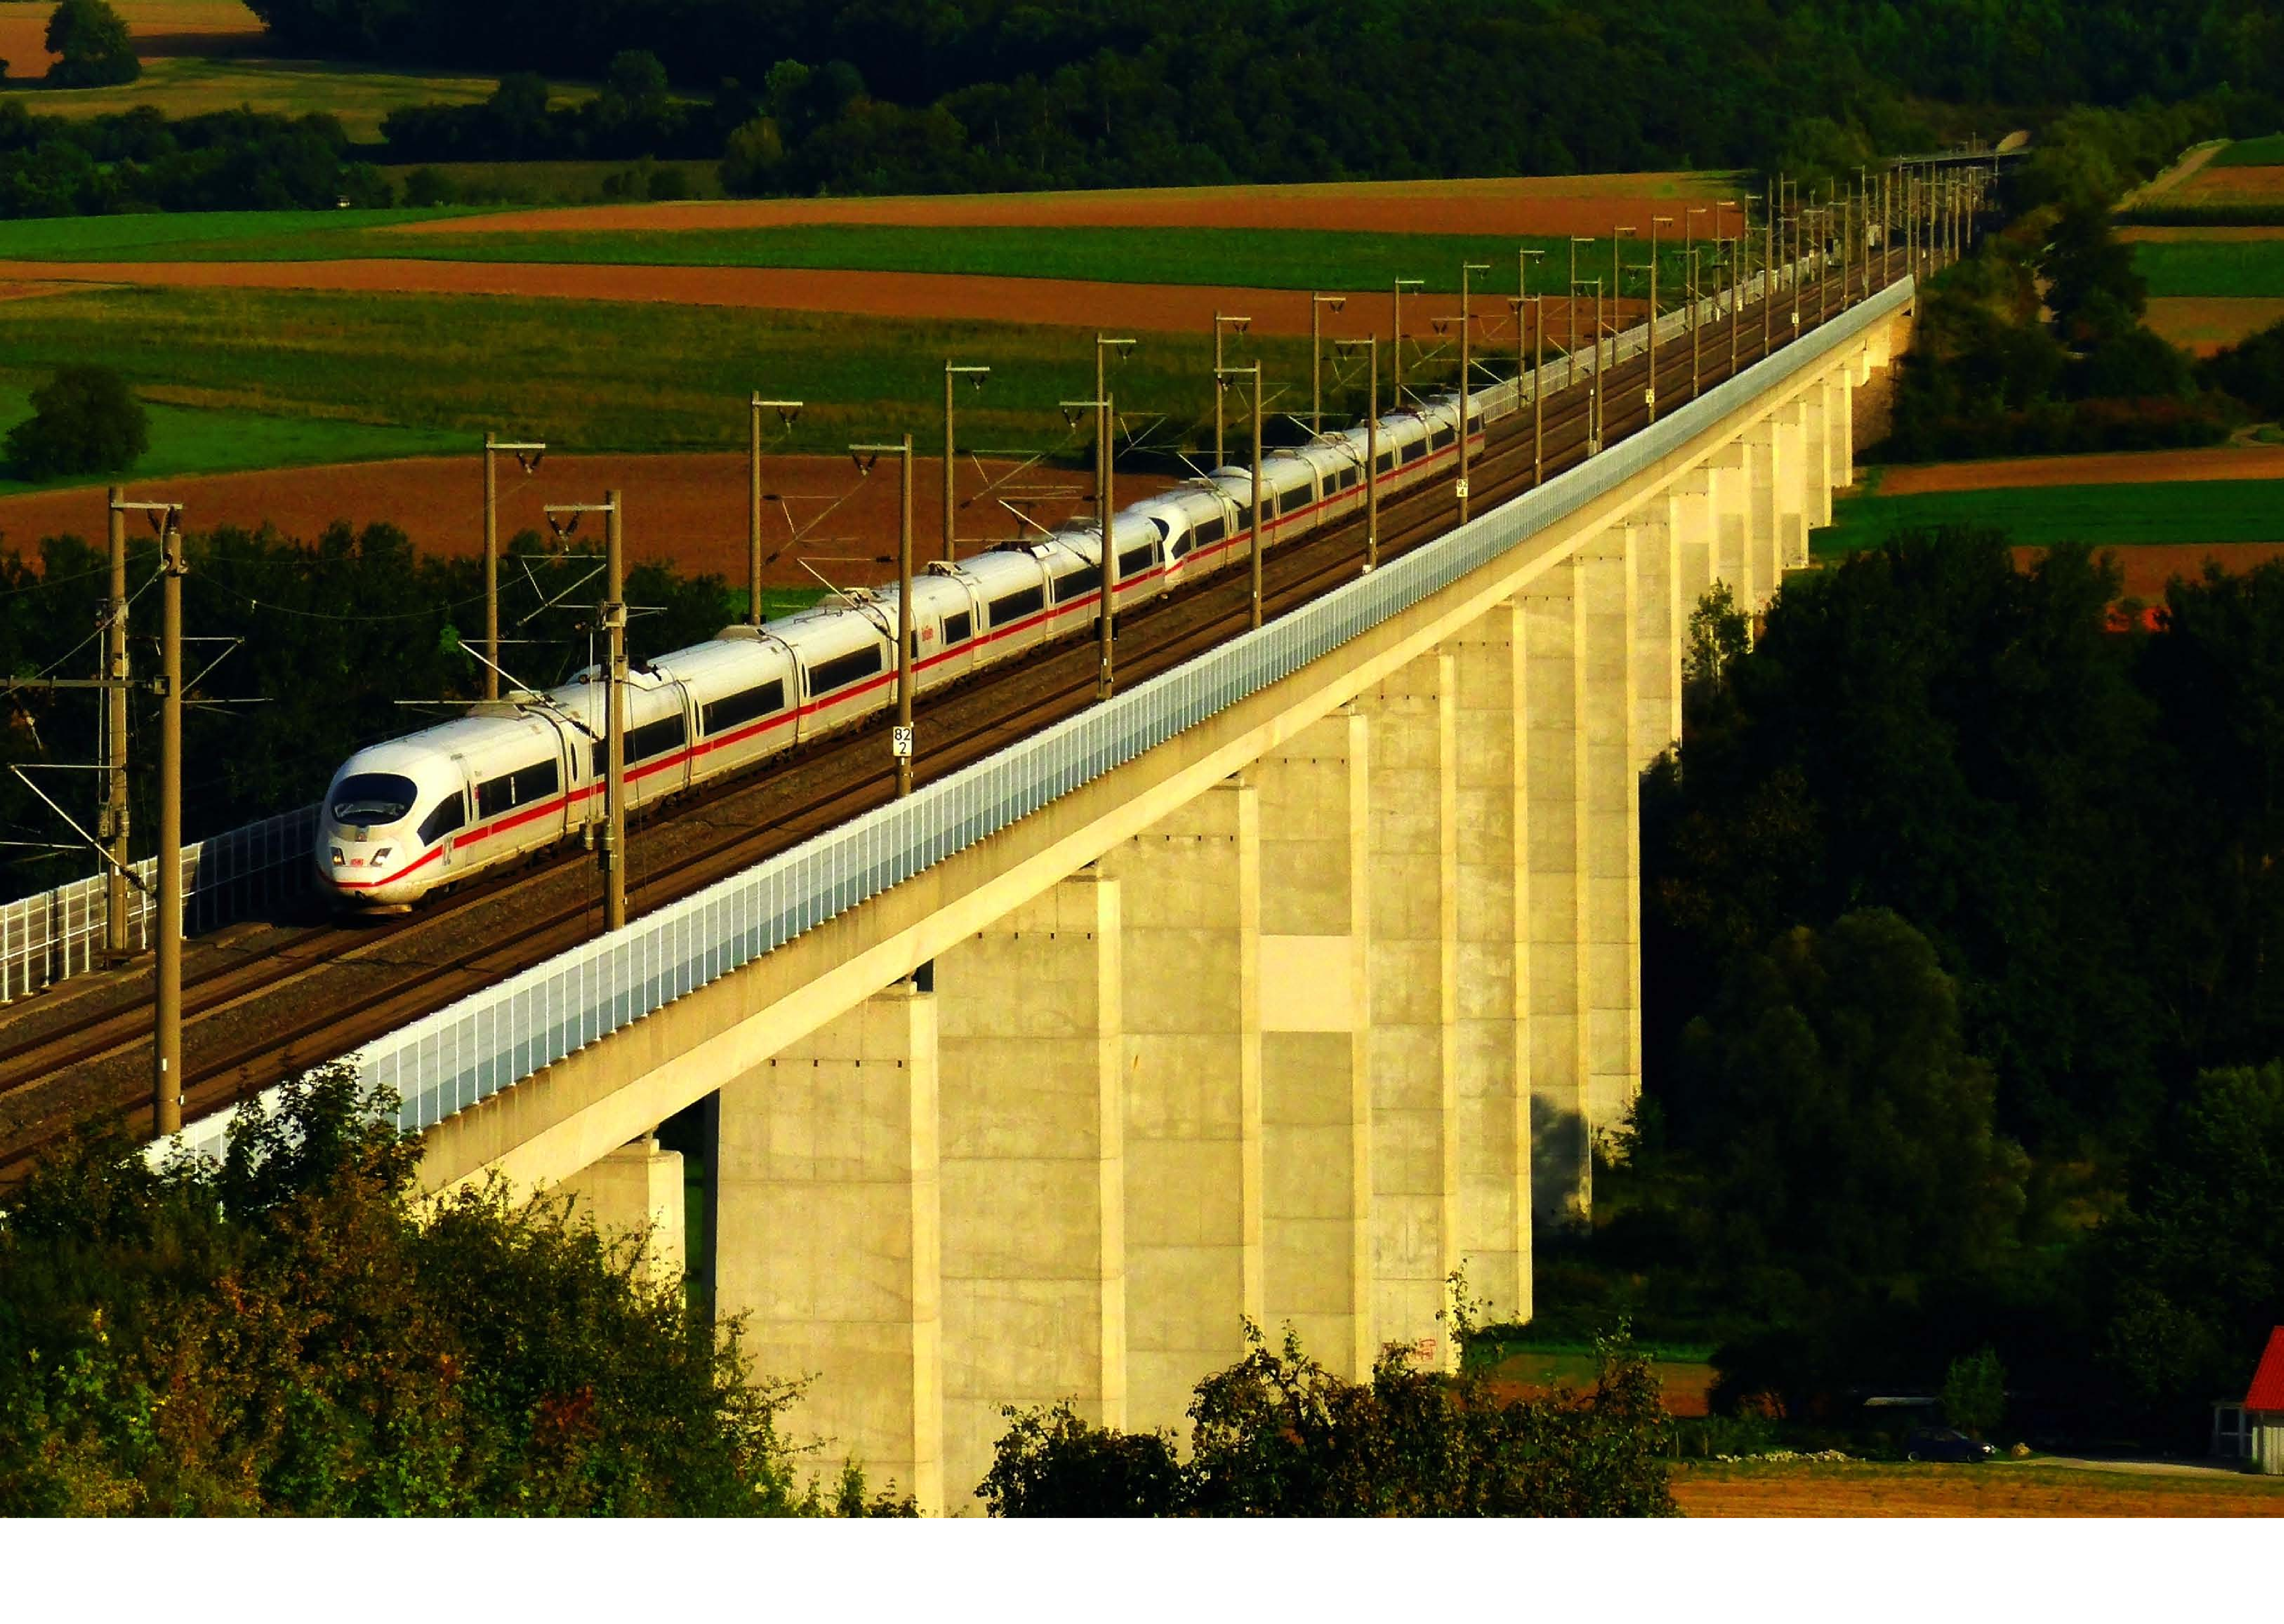
\includegraphics[width=2.5in]{chap2/viaduct.pdf}}
    \hspace{1cm}
\subfigure[隧道]{
    \label{fig:tunnel}
    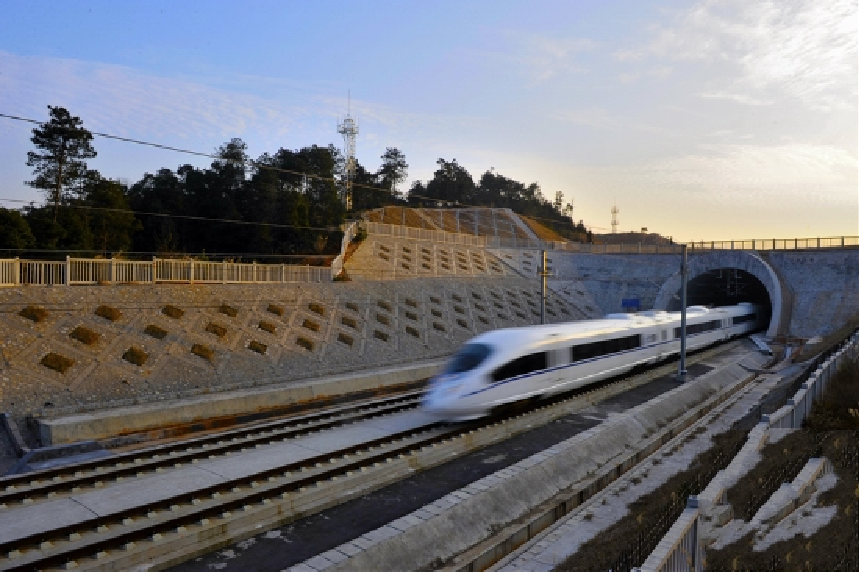
\includegraphics[width=2.5in]{chap2/tunnel.pdf}}
\hspace{1in}
\centering
\subfigure[山区]{
    \label{fig:mountain}
    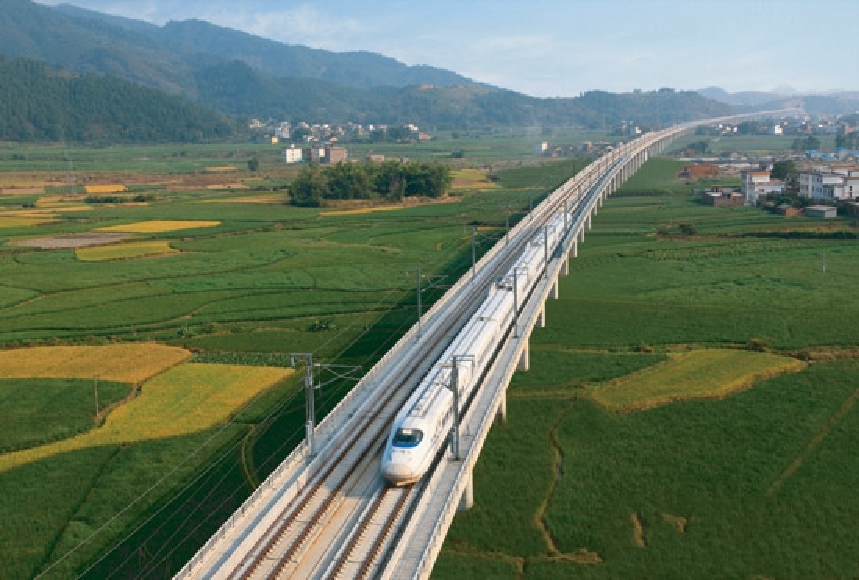
\includegraphics[width=2.5in]{chap2/mountain.pdf}}
    \hspace{1cm}
\subfigure[平原]{
    \label{fig:plain}
    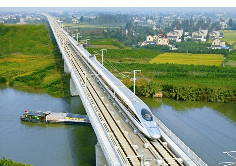
\includegraphics[width=2.5in]{chap2/plain.pdf}}
%\hspace{1in}
%\centering
%\subfigure[车站]{
%    \label{fig:hongqiao}
%    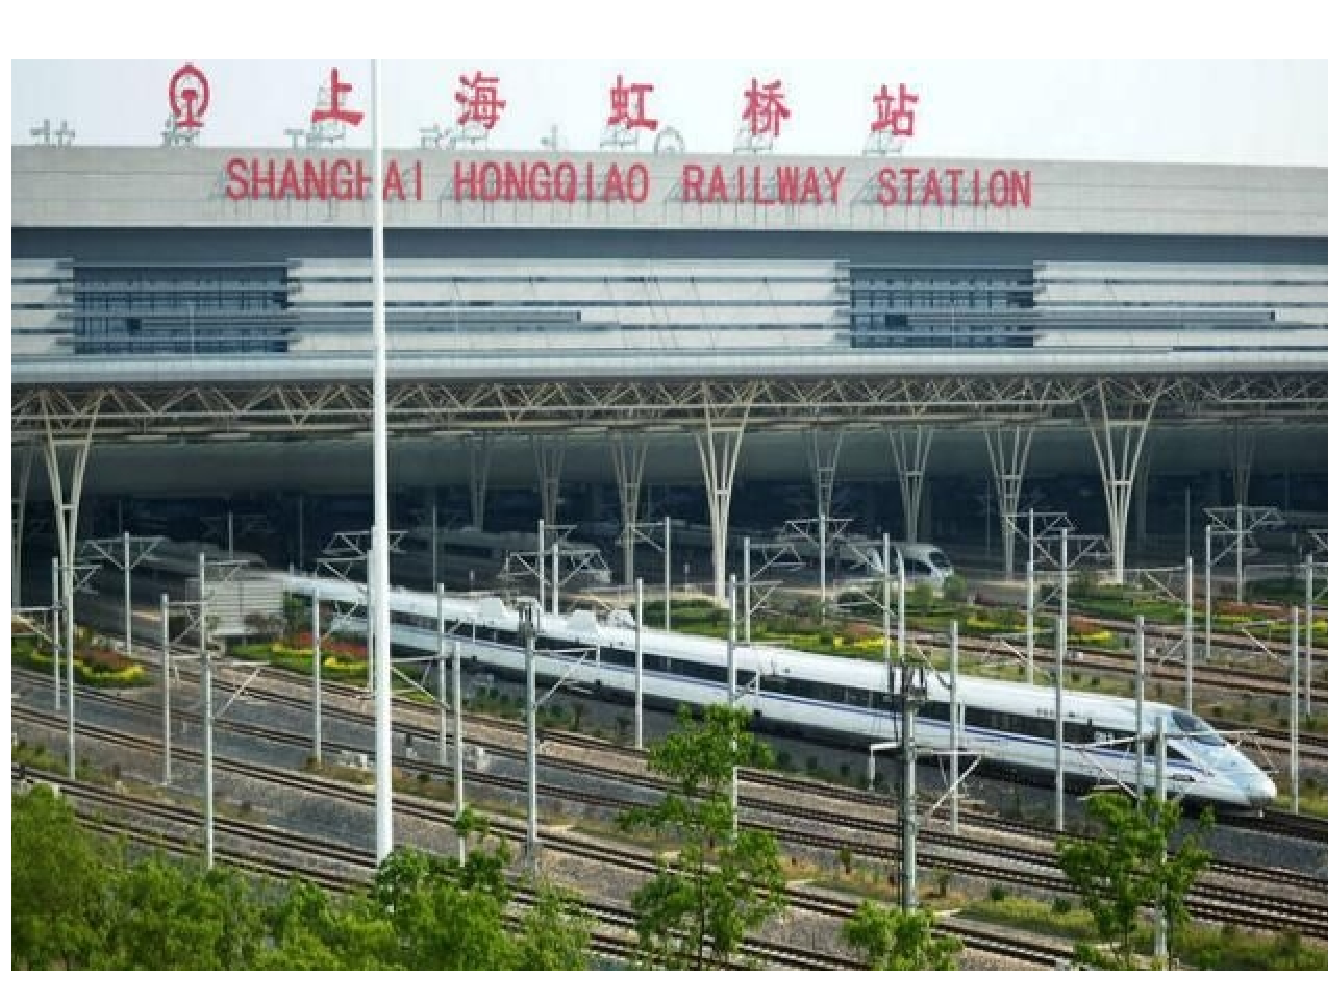
\includegraphics[width=2.5in]{chap2/hongqiao.pdf}}
%    \hspace{1cm}
%\subfigure[基站]{
%    \label{fig:qingzang}
%    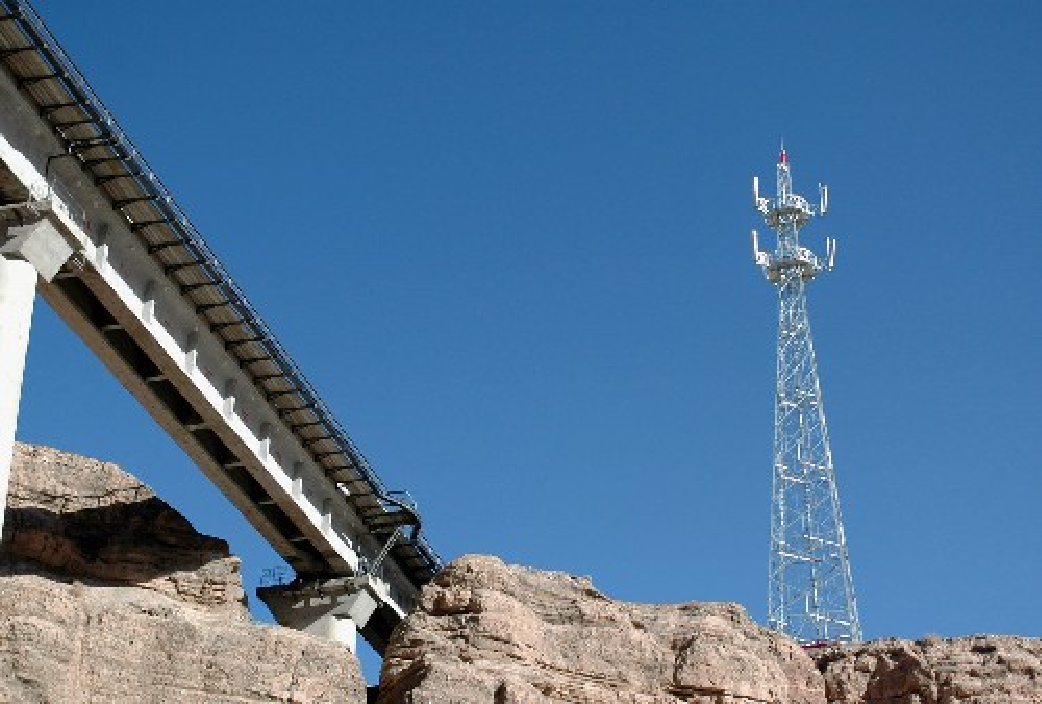
\includegraphics[width=2.5in]{chap2/qingzang.pdf}}
\bicaption[fig:terrain]{GSM-R网络无线传播环境}{GSM-R网络无线传播环境}{Fig}{Radio Propagation Environments and terrains of GSM-R Networks}
\end{figure}

在GSM-R网络空中接口的无线通信中,接收信号强度可以视为阴影衰落与多径衰落的叠加,如式(\ref{equa:p_r1})所示,
\begin{equation}
    p_{r}^{2}(x) = s(x)h(x)
\label{equa:p_r1}
\end{equation}
其中$s(x)$为阴影衰落,服从高斯过程;$h(x)$为多径衰落,服从复高斯过程;$x$可以视为移动台与基站之间距离,利用列车运行速度公式可以转化为时间变量。如图 \ref{fig:train} 所示,GSM-R网络中移动台与基站间距离$d$在10m左右,因此$\Delta x=\sqrt{d^2+v_{train}^2\cdot \Delta t^2}$ 可以简化为$\Delta x=v_{train}\cdot \Delta t$。同时式(\ref{equa:p_r1})可以表示为对数域形式,如式(\ref{equa:P_r2})所示,
\begin{equation}
P_{r}(x) = S(x) + H(x)
\label{equa:P_r2}
\end{equation}
其中$P_r(x)$、$S(x)$、$H(x)$分别为接收功率与信号衰落在对数域的表示,即$P_r(x):=10\log(p_{r}^{2}(x))$,$S(x):=10\log(s(x))$,$H(x):=10\log(h(x))$。

\begin{figure}[!htp]
\centering
    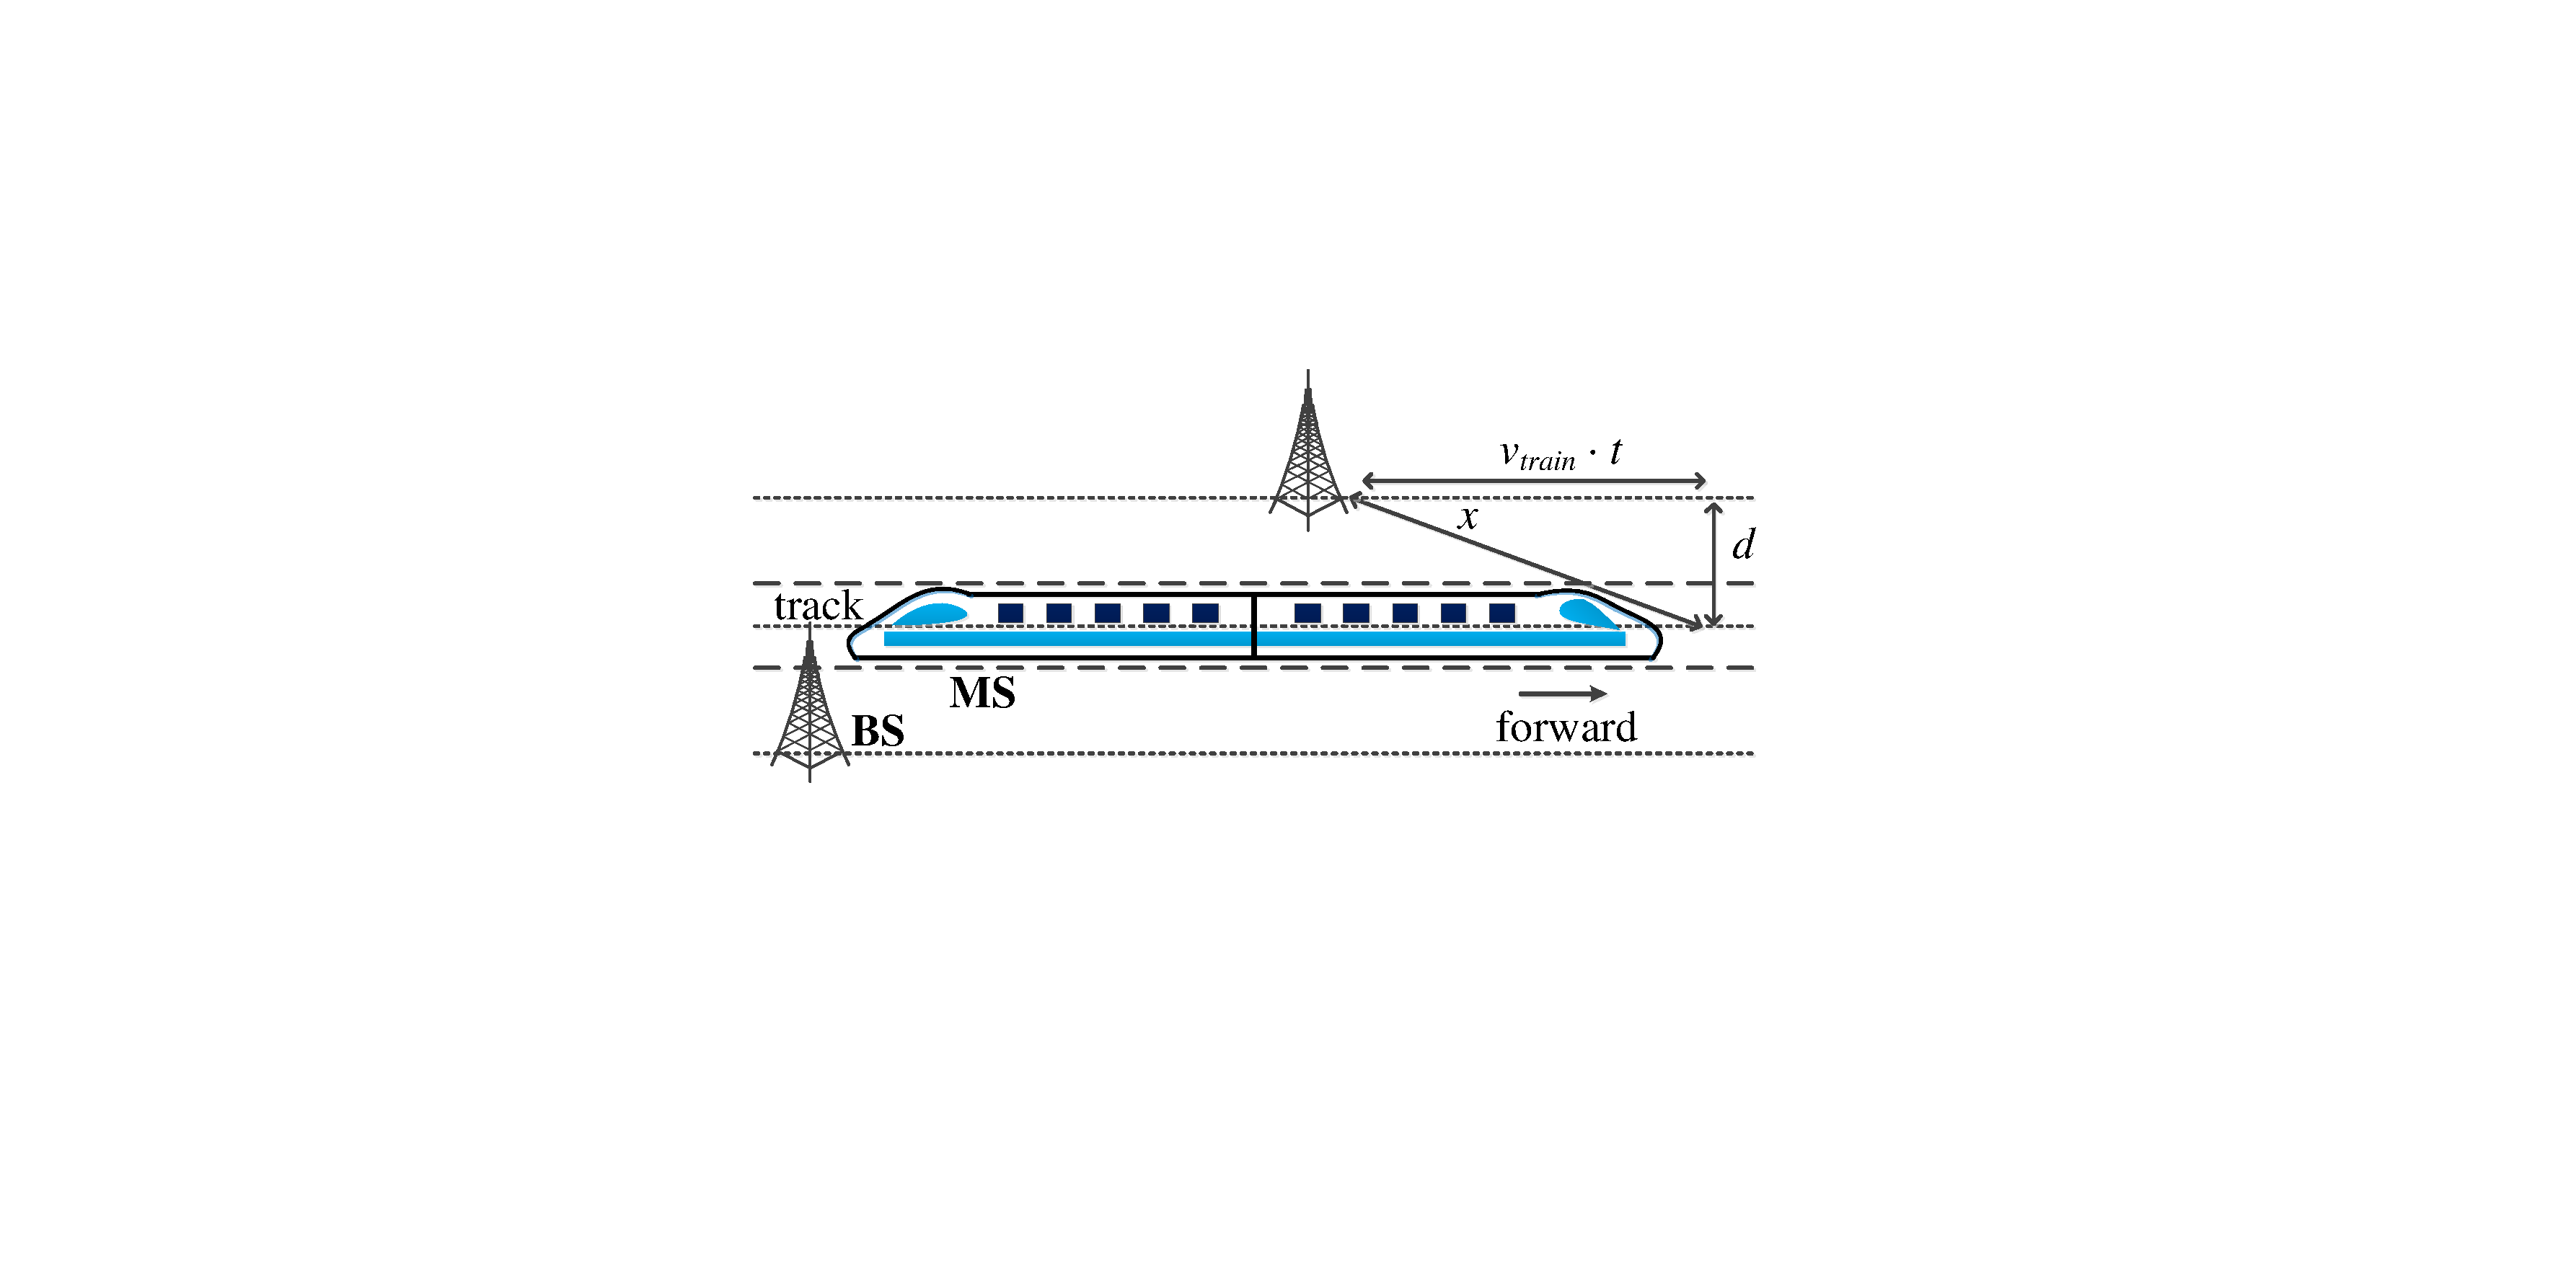
\includegraphics[width=5in]{chap2/train.pdf}
\bicaption[fig:train]{GSM-R网络移动台与基站间距离}{GSM-R网络移动台与基站间距离}{Fig}{The distance between MS and BS in GSM-R networks}
\end{figure}

\subsection{阴影衰落}
\label{sec:shadow}

阴影衰落可用如式(\ref{equa:shadow})所示的高斯过程表示
\begin{equation}
    s(x) \sim N\left( m(x),\sigma_s^2 \right)
\label{equa:shadow}
\end{equation}
其中均值$m(x)$主要受路径损耗影响,方差$\sigma_s^2$受地形因素影响。 文献 \cite{sarkar2003survey} 综合基站发射功率、移动台接收灵敏度以及无线传播环境的影响,给出$m(x)$的基本模型并被广泛应用,表示为式(\ref{equa:pathloss})
\begin{equation}
    M(x)= K_1+K_2\log(x)
\label{equa:pathloss}
\end{equation}
其中$M(x):=20\log(m(x))$为$m(x)$的对数形式,$K_1$主要与基站发射功率、天线增益及线路损耗有关,$K_2$为地形因子并随着无线传播环境的不同而变化 \cite{hata1980empirical} \cite{medeisis2000use}。$S(x)$的空间相关性,即其自相关函数,主要与地形因素有关,表示为式(\ref{equa:multipath}) \cite{gudmundson1991correlation}。
\begin{equation}
    R_{s}(x) = \sigma_{s}^2\exp\left(-\frac{\Delta x}{x_0}\right)
\label{equa:multipath}
\end{equation}
其中$\sigma_s$为$S(x)$的方差,通常在4到12dB间取值;$x_0$为相关距离,根据传播环境的不同一般为10m到500m \cite{tepedelenlio?lu2001estimation};$\Delta x$为相对距离,可以通过移动台运行速度即采样时间间隔获得,即$\Delta x = v_{train}\cdot\Delta t$。在阴影衰落模型中,地形因子$K_2$、阴影衰落方差$\sigma_s$及自相关距离$x_0$都与无线传播环境有关,同时影响到上层应用的参数设置,例如小区切换算法中的切换门限值的选择。

\subsection{多径衰落}
\label{sec:multipath}

多径衰落是由于信号的衍射和散射而导致的接收信号强度的瞬时波动,所以移动终端的接收信号强度是来自不同方向信号的叠加。由于信号的相位是随机的,因此可以描述为本地均值与噪声信号的总和。由于GSM-R网络的小区半径通常较短,同时无线传播环境一般是平坦的地形,因此多路径衰落包含一个可视LOS信号,此时多径衰落可以刻画为莱斯衰落,表示为可视LOS信号与非直射NLOS信号的叠加,如式(\ref{equa:rician})所示,
\begin{equation}
  h(x)=\underbrace{\frac{1}{\sqrt{1+K}}\lim_{M \to \infty}\frac{1}{\sqrt M}\sum_{m=1}^{M}a_{m}e^{j(\frac{2\pi}{\lambda}\cos(\theta_{m}x)+\phi_m)}}_{\rm NLOS~Components}
  +\underbrace{\sqrt{\frac{K}{1+K}}e^{j(\frac{2\pi}{\lambda}\cos(\theta_{0}x+ \phi_0))}}_{\rm LOS~Component}
\label{equa:rician}
\end{equation}
%\begin{equation}
%\begin{split}
%  h(x)=&\underbrace{\frac{1}{\sqrt{1+K}}\lim_{M \to \infty}\frac{1}{\sqrt M}\sum_{m=1}^{M}a_{m}e^{j\left(\frac{2\pi}{\lambda}\cos(\theta_{m}x)+\phi_m\right)}}_{\rm NLOS~Components}\\
%  &+\underbrace{\sqrt{\frac{K}{1+K}}e^{j(\frac{2\pi}{\lambda}\cos(\theta_{0}x+ \phi_0))}}_{\rm LOS~Component}
%\end{split}
%\label{rician}
%\end{equation}
其中$M$散射信号数量,$\lambda$为信号波长,$\theta_m(m=0,1,...M)$代表不同信号与接收移动终端间夹角,$\phi_m(m=0,1,...M)$为每路信号的相位。在莱斯衰落中,直射路径与非直射路径信号强度分别表示为$\nu^2$和$2\sigma^2$,则$K$表示直射路径信号与其他路径信号的比值,即$K=\nu^2/2\sigma^2$,此时接收信号幅值服从参数为$\nu^2$和$\sigma^2$的莱斯分布,其概率分布函数(Probability Distribution Function, PDF)表示为
\begin{equation}
    f(y;\sigma,\nu)=\frac{y}{\sigma^2}e^{-\frac{y^2+\nu^2}{2\sigma^2}}I_0\left(\frac{y\nu}{\sigma^2}\right)
\label{equa:ricianPDF}
\end{equation}
其中$I_0(\cdot)$零阶第一类修正贝塞尔函数。当不存在直射路径信号,即$K=0$时,莱斯衰落退化为瑞利衰落,此时接收信号幅值的概率分布函数简化为
\begin{equation}
    h(x)=\lim_{M \to \infty}\frac{1}{\sqrt M}\sum_{m=1}^{M}a_{m}e^{j\left(\frac{2\pi}{\lambda}\cos(\theta_{m}x)+\phi_m\right)}
\label{equa:rayleigh}
\end{equation}
\begin{equation}
    f(y;\sigma)=\frac{y}{\sigma^2}e^{-\frac{y^2}{2\sigma^2}}
\label{equa:rayleighPDF}
\end{equation}


\section{信道状态动态估计}
\label{sec:dynamic}

由于GSM-R网络负责为高速铁路提供无线通信,因此需要在线实时测试以保证通信网络与高铁系统的安全可靠运行,本文提出接收信号强度在线动态测试算法,以提高信道状态测试的精度并降低其开销。

\begin{figure}[!htp]
\centering
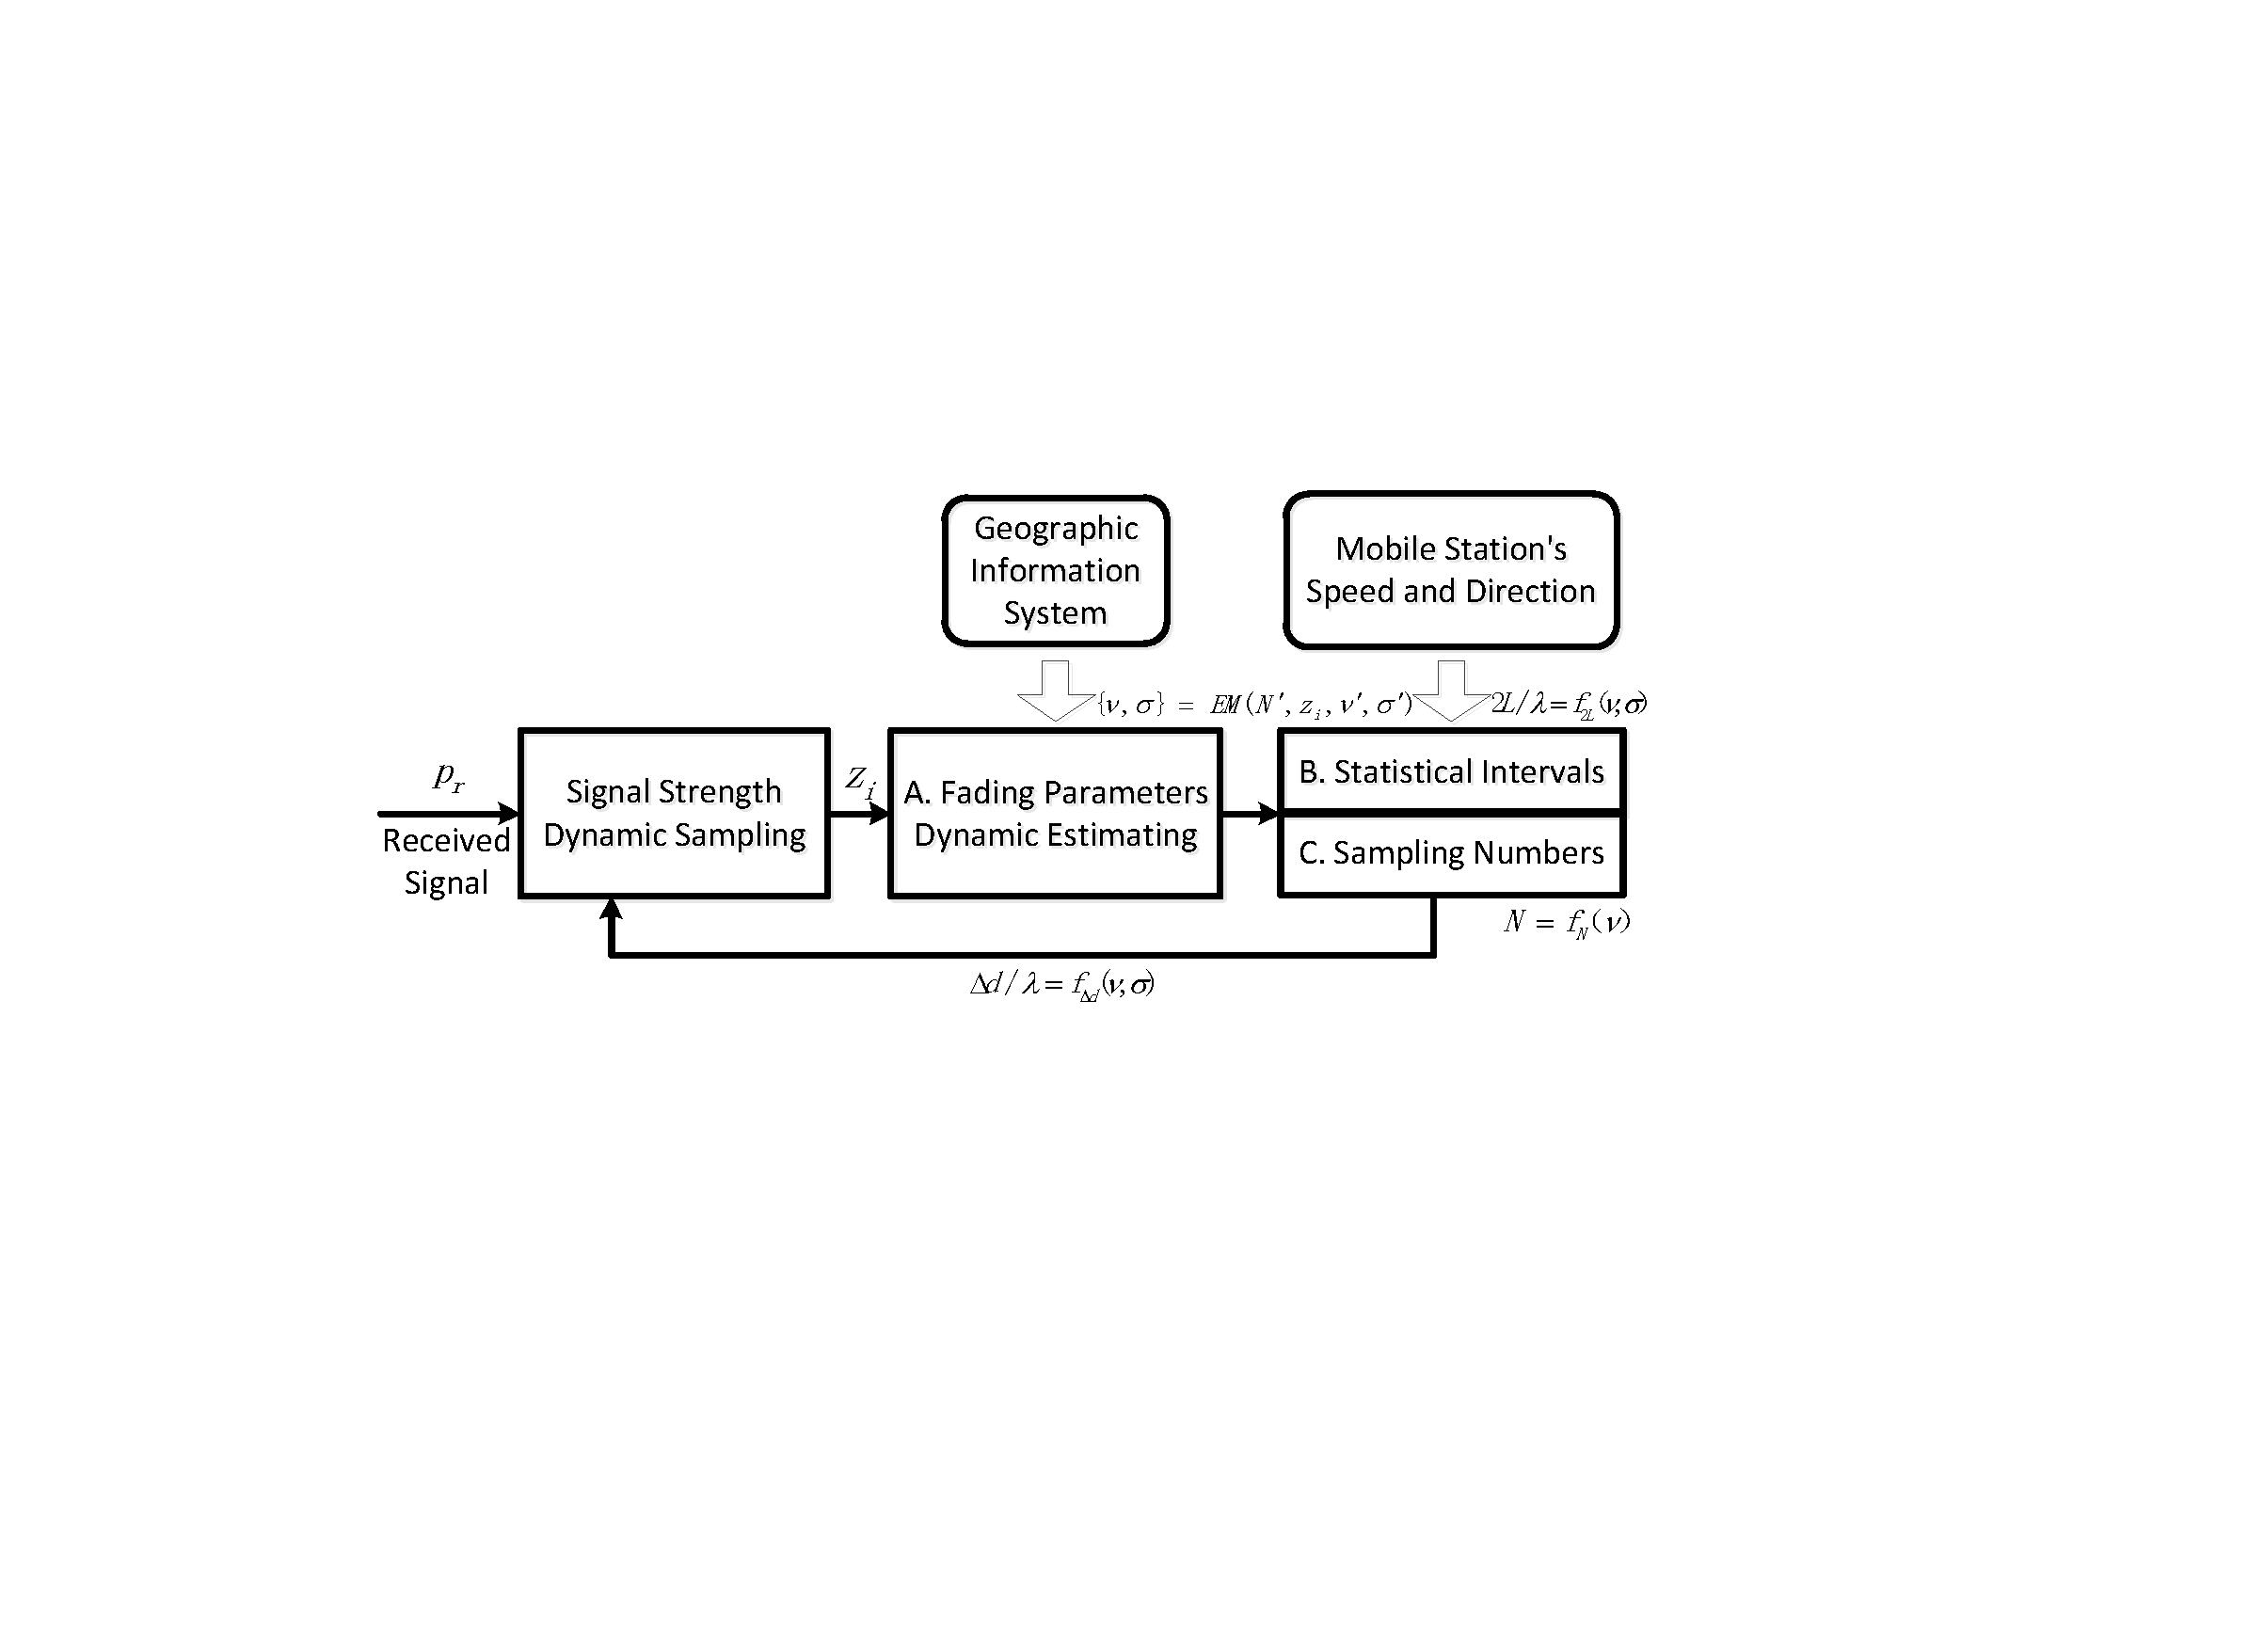
\includegraphics[width=5in]{chap2/online.pdf}
\bicaption[fig:online_measure]{在线动态测试框架}{在线动态测试框架}{Fig}{On-line and Dynamic Estimation of Rician Fading Channels}
\end{figure}

动态测试算法的工作过程如图 \ref{fig:online_measure} 所示,首先对信号进行动态采样,得到一组当前时刻的信号强度值,然后经过衰落参数动态估计,得到当前无线传播环境的莱斯衰落参数,然后经过计算得到统计区间与采样点数,同时以此为基础开始下一次信号采样。

\subsection{信道参数估计}
\label{sec:estimation}

对于莱斯衰落信道的参数估计已有大量相关工作,包括基于学习训练机制 \cite{bjornson2010framework}、最大似然估计 \cite{sijbers1998maximum} 以及期望最大化算法\cite{marzetta1995algorithm}。由于EM算法通过迭代方式进行参数估计,本文采用EM算法进行莱斯参数估计,以充分利用历史信息提高测试精度并降低测试开销。EM算法中莱斯衰落因子$\nu^2$和$\sigma^2$通过其上一时刻估计值与当前采样信号计算获得,如式(\ref{equa:EM})所示
\begin{subequations}
  \begin{eqnarray}
    \nu_{k+1}&=&\frac{1}{N}\sum_{i=1}^{N}\frac{I_{1}\left(\frac{\nu_{k}z_{i}}{\sigma_k^2}\right)}{I_{0}\left(\frac{\nu_{k}z_{i}}{\sigma_k^2}\right)}z_i \\
    \sigma_{k+1}^2&=&\max{\left[\frac{1}{2N}\sum_{i=1}^N z_i^2 -\frac{\nu_k^2}{2},0\right]}
  \end{eqnarray}
\label{equa:EM}
\end{subequations}
其中$I_1(\cdot)$一阶第一类修正贝塞尔函数,$N$为采样信号数码,$\nu_k$和$\sigma_k$为上一时刻估计结果,其初始值为
\begin{subequations}
  \begin{eqnarray}
    \nu_{0}&=& \left(2\left(\frac{1}{N}\sum_{i=1}^N z_i^2\right)^2-\frac{1}{N}\sum_{i=1}^N z_i^4\right)^{1/4} \\
    \sigma_{0}^2&=&\frac{1}{2}\left(\frac{1}{N}\sum_{i=1}^N z_i^2 - \nu_{0}\right)
  \end{eqnarray}
\label{equa:EM0}
\end{subequations}

基于以上的莱斯衰落参数估计,接收信号强度测试的采样频率可以计算得到,表示为信号波长$\lambda$与衰落参数$\nu$和$\sigma$的函数。采样频率$\Delta d$ 通过统计区间长度$2L$与采样点数目$N$的比值计算而来。

\subsection{统计区间长度}
\label{sec:length}

对于第 \ref{sec:channelmodel} 节的无线传播模型,接收信号强度的本地均值通过对采样信号$p_r(x)$在统计区间$2L$内进行积分平均获得,即
\begin{equation}
    \hat{s}=\frac{1}{2L}\int\limits_{y-L}^{y+L} p_r^2(x)dx=\frac{s}{2L}\int\limits_{y-L}^{y+L} h(x)dx
\label{equa:shadowmean}
\end{equation}

如果能够选取合适的统计区间长度$2L$,则估计值$\hat{s}$将逼近其实际值$s$,即$\hat{s}\rightarrow s$,此时小尺度衰落的均值表示为
\begin{equation}
\frac{1}{2L}\int\limits_{y-L}^{y+L} h(x)dx \rightarrow 1
\label{equa:shortterm}
\end{equation}

由式(\ref{equa:shadowmean})可知,估计值$\hat{s}$相对于真实值$s$的误差可以由$\hat{s}$的方差衡量,如式(\ref{equa:shadowvariance})所示
\begin{equation}
    \sigma_{\hat{s}}^{2}=\frac{1}{L}\int\limits_{0}^{2L}\left(1-\frac{\tau}{2L}\right)R_{p_{r}^2}(\tau)d\tau
\label{equa:shadowvariance}
\end{equation}
其中$R_{p_{r}^2}(\tau)=E[p_{r}^{2}(x)p_{r}^{2}(x+\tau)]-E[p_{r}^{2}(x)]E[p_{r}^{2}(x+\tau)]$为包络信号$p_{r}(x)$的自相关函数。则估计值$\hat{s}$的均一化误差可以表示为
\begin{equation}
P_e:=10 \log_{10}\left(\frac{\hat{s}+\sigma_{\hat{s}}}{\hat{s}-\sigma_{\hat{s}}}\right)
\label{equa:perror}
\end{equation}

\begin{figure}[!htp]
  \centering
  \subfigure[$\sigma=1$]{
    \label{fig:sigma1}
    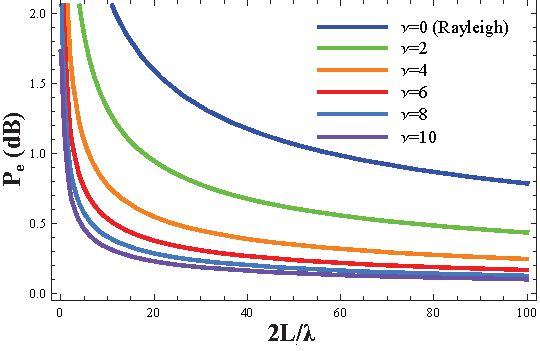
\includegraphics[width=2.5in]{chap2/sigma11.pdf}}
    \hspace{1cm}
  \subfigure[$\sigma=3$]{
    \label{fig:sigma3}
    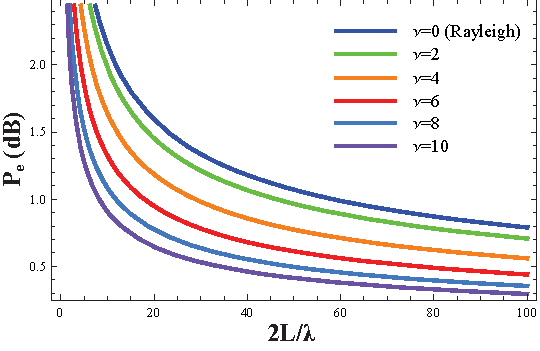
\includegraphics[width=2.5in]{chap2/sigma33.pdf}}
  \hspace{1in}
  \centering
  \subfigure[$\sigma=5$]{
    \label{fig:sigma5}
    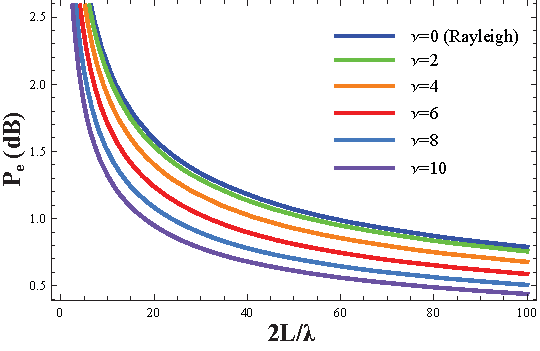
\includegraphics[width=2.5in]{chap2/sigma55.pdf}}
    \hspace{1cm}
  \subfigure[$\sigma=7$]{
    \label{fig:sigma7}
    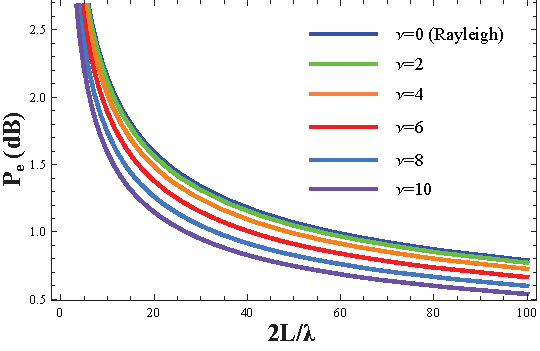
\includegraphics[width=2.5in]{chap2/sigma77.pdf}}
  \bicaption[fig:length]{统计区间长度}{统计区间长度}{Fig}{Proper Length of Statistical Intervals}
\end{figure}

将式(\ref{equa:shadowmean})和式(\ref{equa:shadowvariance})带入式(\ref{equa:perror})中,并按照附录\ref{appsec:lengthestimation}求解积分方程,归一化误差$P_e$可以表示为
\begin{equation}
P_e = 10 \log_{10}\left(\frac{\frac{2\sigma^2+\nu^2}{2\sigma^2}n+\sqrt{2(1+n)\int\limits_0^n g\left(\frac{\nu^2}{2\sigma^2};\rho\right) d\rho}}{\frac{2\sigma^2+\nu^2}{2\sigma^2}n-\sqrt{2(1+n)\int\limits_0^n g\left(\frac{\nu^2}{2\sigma^2};\rho\right) d\rho}}\right)
\label{equa:Perror}
\end{equation}
其中$\nu$和$\sigma$为莱斯衰落信道参数。令归一化误差等于1,即$P_e=1dB$,则可以得到合适的统计区间长度$2L$与信号波长$\lambda$及衰落参数$\nu^2$和$\sigma^2$的关系式,即$2L=f_{2L}(\lambda;\nu,\sigma)$或$2L/\lambda=f_{2L/\lambda}(\nu,\sigma)$,如图 \ref{fig:length} 所示。

\subsection{采样点数}
\label{sec:number}

除了选择合适的统计区间长度外,还需要确定采样点数目,以有效降低多径衰落对信号估计的影响。采样得到的接收信号功率可以通过衰落参数计算得到,结合式(\ref{equa:EM})有$r^2=2\sigma^2+\nu^2\approx\frac{1}{N}\sum_{i=1}^N z_i^2$,则$r^2$的估计值及其方差为
\begin{subequations}
  \begin{eqnarray}
    \bar{r^2}&=&E\left[r^2\right]=\frac{1}{N}E\left[\sum_{i=1}^{N}z_i^2\right] \\
    \sigma_{\bar{r^2}}&=&D\left[r^2\right]=\frac{1}{N^2}D\left[\sum_{i=1}^{N}z_i^2\right]
  \end{eqnarray}
\label{equa:number}
\end{subequations}

与统计区间长度的归一化误差类似,采样点数目的归一化误差为
\begin{equation}
Q_e=10 \log_{10}\left(\frac{\bar{r^2}+\sigma_{\bar{r^2}}}{\bar{r^2}}\right)
\label{equa:qerror}
\end{equation}

\begin{figure}[!htp]
\centerline{
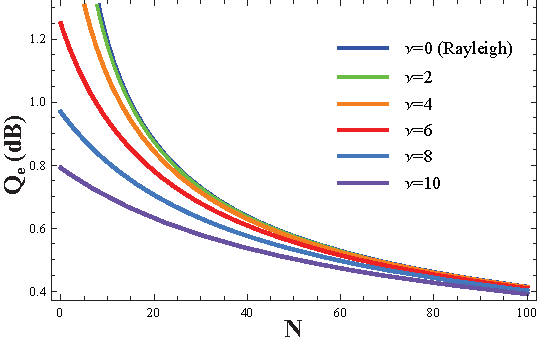
\includegraphics[width=4.0in]{chap2/nu1.pdf}
}
\bicaption[fig:nu]{采样点数}{采样点数}{Fig}{Required Number of Averaging Samples}
\end{figure}

根据附录 \ref{appsec:numberestimation} 中的计算与推导,$Q_e$可以表示为
\begin{equation}
    Q_e=10 \log_{10}\left(\frac{2N+\nu^2+2\sqrt{N+\nu^2}}{2N+\nu^2}\right)
\label{equa:Qerror}
\end{equation}
其中$\nu$和$\sigma$为莱斯衰落参数,通过如式(\ref{equa:EM})中EM算法计算得到。显然采样点数目只与莱斯衰落参数$\nu$有关,即$N=f_{N}(\nu)$,如图 \ref{fig:nu} 所示。

接收信号强度采样频率$\Delta d$由$2L/N$计算获得,即$\Delta d=f_{2L}(\lambda;\nu,\sigma)/f_{N}(\nu)=f_{\Delta d}(\lambda;\nu,\sigma)$。 由于信号波长$\lambda$在通信过程中一般保持不变,因此$\Delta d$与莱斯衰落参数$\nu$和$\sigma$密切相关。

\section{系统实现}
\label{sec:system_phy}

GSM-R网络通信质量测试系统主要完成物理指标的实时测量,同时对网络链路质量进行统计与分析,包括实时测试与离线分析。GSM-R网络空中接口测试系统实现对GSM-R网络通信质量的在线实时与离线综合测试,如图 \ref{fig:umsystem} 所示。在线测试实现对GSM-R网络通信质量的实时监测,同时在网络出现故障时给出预警信息;离线测试对GSM-R网络性能进行统计与分析,给出网络的综合性能评估,并提出参数调整建议。同时测试指标包含网络物理层、链路层与业务层各项指标,实现对GSM-R网络通信质量的全面测试,保证高铁系统的安全稳定高速运行。

本章首先引入GSM-R网络空中接口测试系统的基本结构,包括硬件平台与软件开发,然后分析动态测试算法的设计与实现,最后对系统的基本功能进行简单介绍。

\subsection{硬件平台}
\label{sec:um}

GSM-R网络测试系统由无线收发模块、通信协议处理模块、数据分析处理模块构成,如图 \ref{fig:umhardware} 所示,其中无线收发模块完成GSM-R网络通信信号采集,通信协议处理模块主要对采集到的网络信令进行解析,数据分析处理模块负责对网络各项性能指标进行统计与分析。

测试系统中心处理器模块为美国RTD公司的CME137686LX-W cpuModules™,通信协议处理模块与射频收发模块选择德国Triorail公司的GSM-R网络收发模块TRM:3a,外加RTD公司的GSM-R网络收发模块外围开发板COM16155RER-1,上述模块通过PC/104与RTD的电源模块VPWR104HR-L50W相连接,从而实现GSM-R 网络信息收发功能。

\begin{figure}[!htp]
%\onelinecaptionsfalse
\centering
    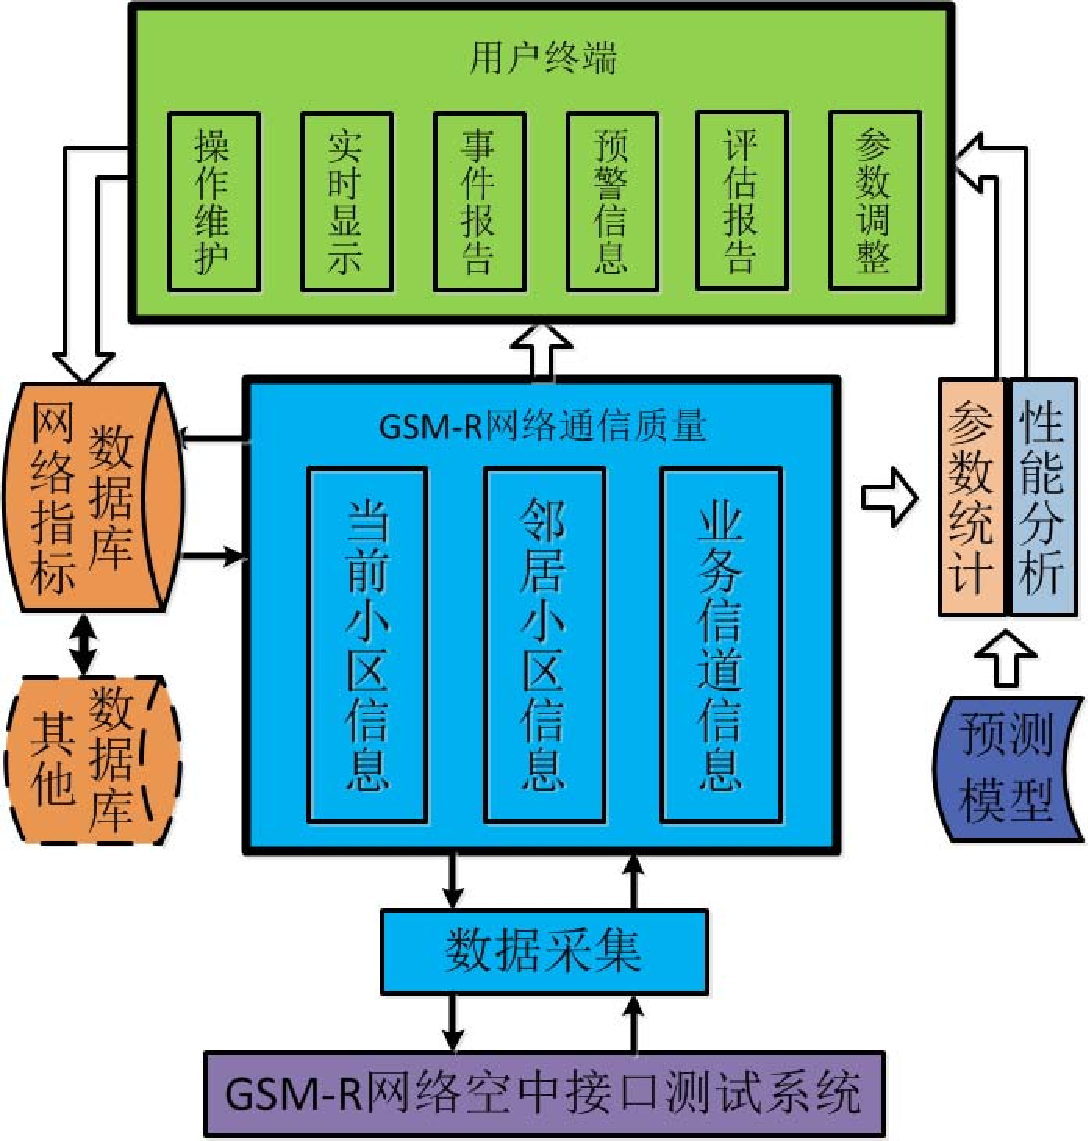
\includegraphics[width=5in]{chap2/softwarefunction.pdf}
\bicaption[fig:umsystem]{GSM-R网络空中接口测试系统}{GSM-R网络空中接口测试系统}{Fig}{Um interface monitoring system for GSM-R networks}
\end{figure}

GSM-R网络空中接口测试系统的硬件平台由PC/104总线实现模块间通信,主要由以下三部分组成:
\begin{itemize}
  \item \textbf{处理器模块}
  处理器模块采用RTD公司符合军工标准的CME137686LX-W模块,该模块采用500MHz AMD™ Geode LX处理器,具有128kB L1缓存和128kB L2缓存,采用333MHz DDR-SDRAM控制器支持最高2.7G-Bytes/s的存储带宽,包括4个USB 2.0 接口, 2个SATA II 接口, 3个串口、千兆以太网口、8GB板贴固态硬盘和8个GPIO,在有效完成数据处理的同时,满足高速铁路复杂的无线传播环境。
  \item \textbf{无线通信模块}
  COM16155ER模块板载Cinterion 4频段GSM/GPRS模块MC55i和Fastrax IT500 GPS模块,在实际测试过程中,将GSM模块替换为德国Triorail公司的GSM-R收发模块TRM:3a。COM16155ER板载两个ISA总线接口的UART,分别连接到GSM-R模块和GPS模块,主机模块通过UART和相关接口对GSM-R模块和GPS模块进行操作。
  \item\textbf{电源模块}
  电源模块采用RTD的电源模块VPWR104HR-L50W,输入电压20-28VDC,输出电压-12V到+19V,工作温度-40到+85C$\circ$,能够满足高速铁路的特殊环境要求。
\end{itemize}

\begin{figure}[!htp]
%\onelinecaptionsfalse
\centering
    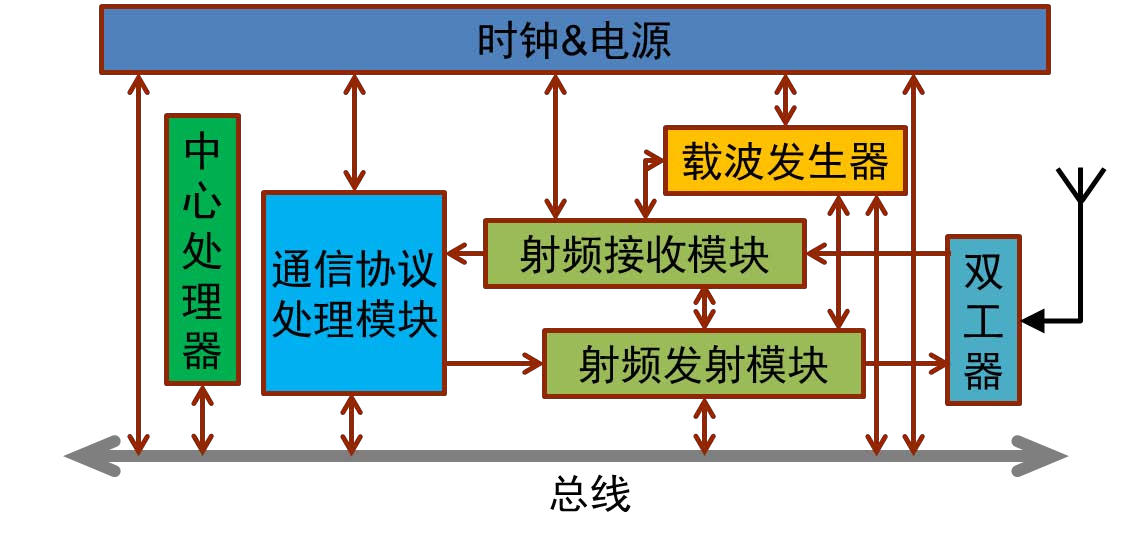
\includegraphics[width=5in]{chap2/hardware.pdf}
\bicaption[fig:umhardware]{GSM-R网络空中接口测试系统硬件组成}{GSM-R网络空中接口测试系统硬件组成}{Fig}{Hardware components of Um interface monitoring system for GSM-R networks}
\end{figure}

上述各模块符合工业级标准,性能稳定并能够工作在各种恶劣环境,同时PC/104作为工业级总线能够保证系统的实时性与可靠性。

\subsection{软件开发}
\label{sec:softwaregsmmr}

GSM-R网络空中接口测试软件平台的开发基于Visual Studio 2008开发环境,开发语言为C\#,软件运行平台为Windows XP、Windows Mobile或Windows CE 操作系统,运行环境Microsoft .NET Compact Framework 2.0或者以上版本,测试系统的启动和运行界面如图 \ref{fig:copyright} 和图 \ref{fig:interface} 所示。

\begin{figure}[!htp]
%\onelinecaptionsfalse
\centering
    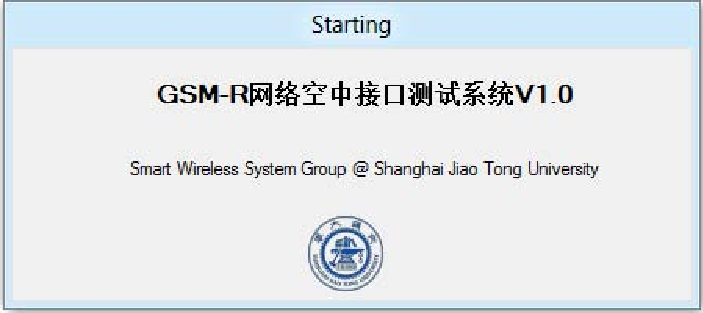
\includegraphics[width=3.2in]{chap2/softwarecopyright.pdf}
\bicaption[fig:copyright]{GSM-R网络空中接口测试系统启动界面}{GSM-R网络空中接口测试系统启动界面}{Fig}{Software starting of Um interface monitoring system for GSM-R networks}
\end{figure}

\begin{figure}[!htp]
%\onelinecaptionsfalse
\centering
    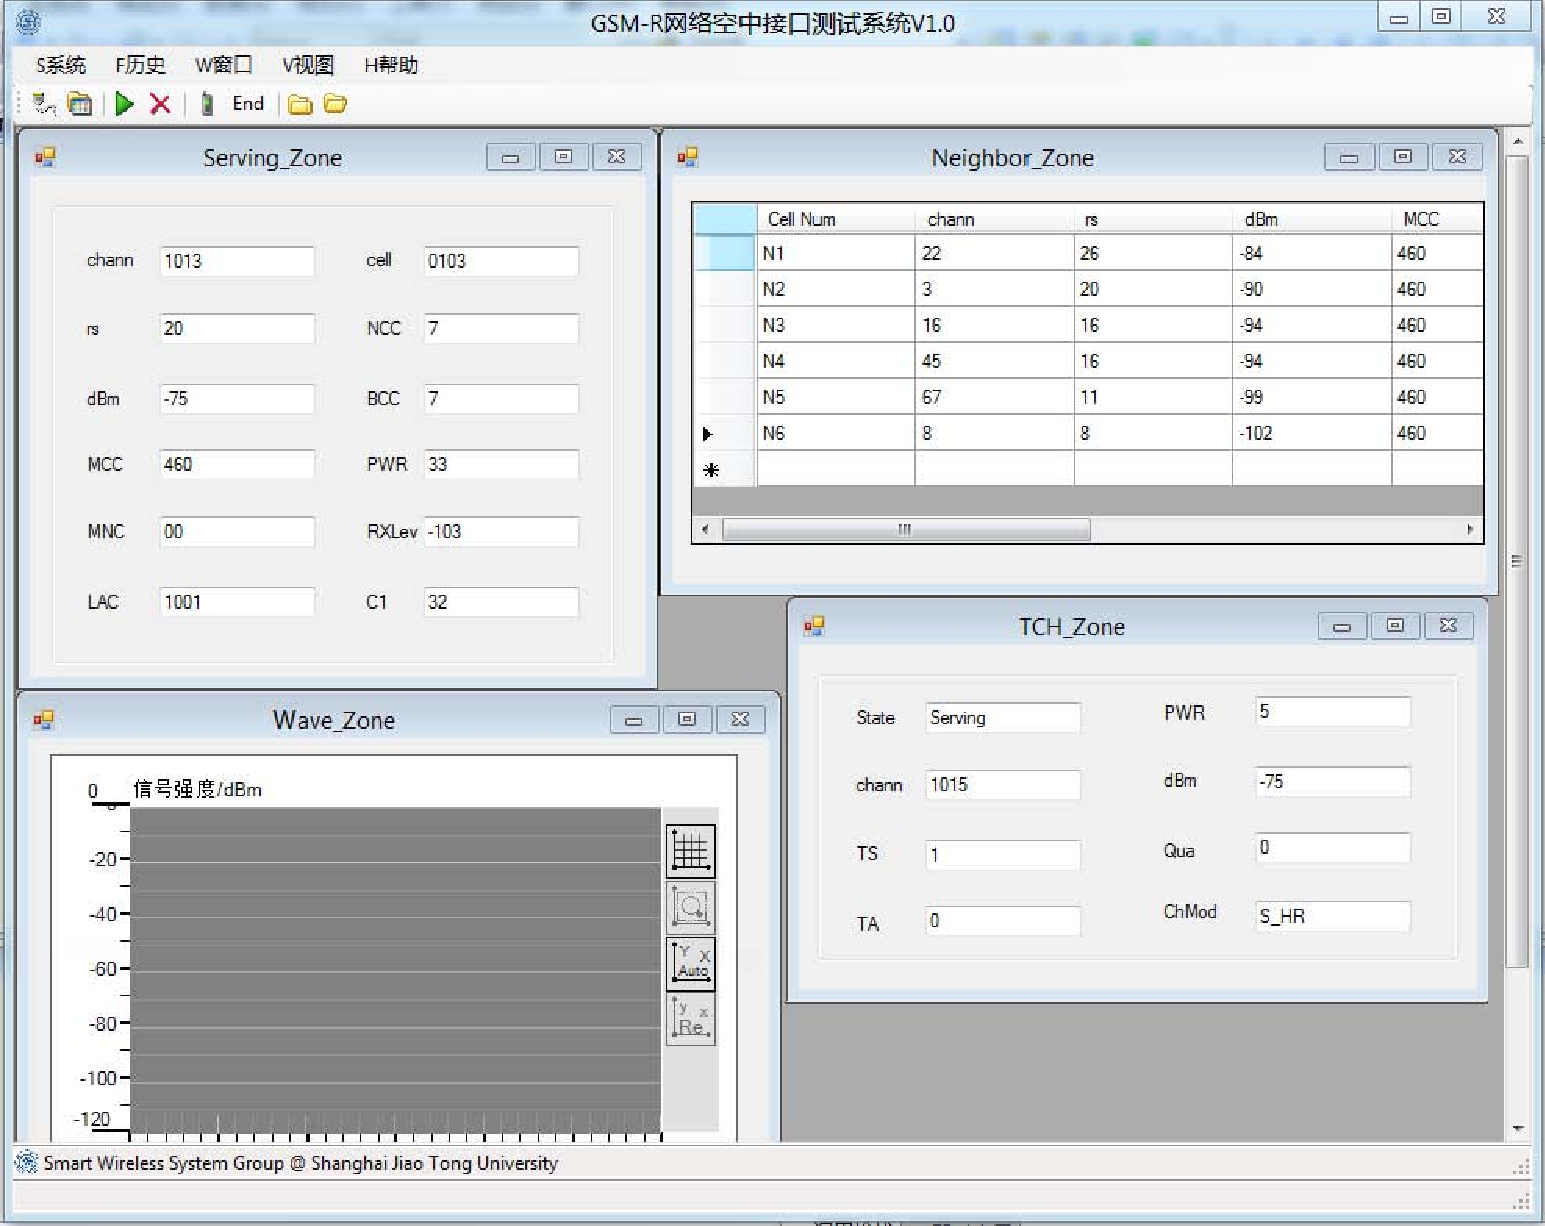
\includegraphics[width=5in]{chap2/softwarestart.pdf}
\bicaption[fig:interface]{GSM-R网络空中接口测试系统软件界面}{GSM-R网络空中接口测试系统软件界面}{Fig}{Software interface of Um interface monitoring system for GSM-R networks}
\end{figure}

该软件平台通过AT命令实现与GSM-R通信模块间的数据交换,主要实现以下信息的测试与分析:

\begin{table}[!htp]
\renewcommand{\arraystretch}{1}
\bicaption[tab:rxlev]{RxLev映射关系}{RxLev映射关系}{Table}{Mapping relation of RxLev}
\centering
\begin{threeparttable}[b]
\begin{tabular}{cc}
\hline
0        & RX < -110 dBm \\
\hline
1        & -110 ≤ RX < -109 dBm \\
\hline
2        & -109 ≤ RX < -108 dBm \\
\hline
3        & -108 ≤ RX < -107 dBm \\
\hline
--- ---      & --- --- \\
\hline
62       & -49 ≤ RX < -48 dBm \\
\hline
63       & RX > -48 dBm \\
\hline
$\leq$17 & 信号强度不满足室外覆盖要求 \\
\hline
$\leq$27 & 信号强度不满足室内覆盖要求 \\
\hline
\end{tabular}
\end{threeparttable}
\end{table}

\begin{enumerate}
  \item 无线信号强度(RxLev):接收到信号电平强度的统计参数,作为功率控制和切换过程的依据,以dBm为单位,接收信号电平被映射到0$\sim$63 之间的某个RxLev值,如表 \ref{tab:rxlev} 所示。
  \item 绝对无线频率信道数(ARFCN):跳频序列的载频号,描述测量数据中的无线载波的变化,阐述了空中接口上下行无线链路。
  \item 接收信号强度指示(RSSI):接收信号强度水平,在这里表示的是在广播控制信道上的接收信号强度水平。
  \item 接收信号强度(dBm):接收信号强度,以dBm为单位,分为广播控制信道和业务信道两种情况。
  \item 小区重选系数(C1\&C2):C1是小区选择时的判断标注,C2是可选参数,仅用于小区重选,若C2未被广播,则使用C1做重选参数。
  \item 时间提前量(TA):补偿电波传输延迟,以提高信道编解码效率。由基站根据测量报告确定,然后发送给手机,当移动台接近基站时减小时间提前量;而当移动台远离小区中心时加大时间提前量。
  \item 信道类型(ChMod):业务信道的传输模式。业务信道承载话音或用户数据,全速率业务信道载有总速率为22.8kbit/s的信息。
  \item 功率等级(PWR):分为接入信道最大功率和当前业务信道的功率。
  \item 基站识别码(BSIC):由基站色码和网络色码组成,用于采用相同载频号码且位置相邻的不同基站的识别。其中网络色码识别相邻国家不同网络,基站色码识别相同载频的相邻基站。
  \item 小区编号(Cell ID)与信道编号(chann):小区编号是区分与同一个基站控制器相连的不同基站收发台,信道编号为广播控制信道载频号。
\end{enumerate}

\subsection{算法实现}
\label{sec:alggsmr}

GSM-R网络接收信号强度在线测试的伪代码如算法 \ref{alg:online} 所示,主要基于第 \ref{sec:dynamic} 章的推导与计算。首先通过EM算法进行莱斯衰落参数估计,实现莱斯衰落因子$\nu_0$和$\sigma_0$的初始化,此时的信号采样参数去瑞利衰落时的参数设置,即统计区间$2L=40\lambda$,采样点数$N=36$。然后在每一轮采样周期基于上一轮估计结果和当前采样信息,对衰落因子$\nu_k$和$\sigma_k$进行实时更新,同时确定下一轮采样参数$2L$和$N$。最后通过统计区间长度和采样点数计算得到采样间隔$\Delta d=2L/N$,并开始新一轮的信号采样与参数估计。

\begin{algorithm}[!htp]
\floatname{algorithm}{算法}
\renewcommand{\algorithmicrequire}{\textbf{输入:}}
\renewcommand{\algorithmicensure}{\textbf{输出:}}
\caption{莱斯衰落信道在线采样与估计}
\label{alg:online}
\begin{algorithmic}[1]
\Require $v_{train}$, $r_i$, $\nu_k$, $\sigma_k$
\Ensure  $\nu_{k+1}$, $\sigma_{k+1}$, $2L$, $N$, $\Delta d$
\State {// 1. 衰落参数$\nu$和$\sigma$初始化}
\If {begin-flag==true}
\State {$\Delta d$ $\leftarrow$ Lee($2L_0$,$N_0$;$\lambda$);}
\State {\{$\nu_{last}$, $\sigma_{last}$\} $\leftarrow$ EM($\Delta d$,$N_0$;$r_i$); // 式(\ref{equa:EM0})}
\State {\{$\nu_{now}$, $\sigma_{now}$\} $\leftarrow$ EM($\Delta d$,$N_0$;$r_i$;$\nu_{last}$,$\sigma_{last}$); // 式(\ref{equa:EM})}
\While {($\nu_{now}-\nu_{last}>\nu_{thr}$) \& ($\sigma_{now}-\sigma_{last}>\sigma_{thr}$)}
\State {\{$\nu_{next}$, $\sigma_{next}$\} $\leftarrow$ EM($\Delta d$,$N_0$;$r_i$;$\nu_{now}$,$\sigma_{now}$); // 式(\ref{equa:EM})}
\State {$\{\nu_{last},\sigma_{last}\} \leftarrow \{\nu_{now},\sigma_{now}\}$;}
\State {$\{\nu_{now},\sigma_{now}\} \leftarrow \{\nu_{next},\sigma_{next}\}$;}
\EndWhile
\State {$2L_{now} \leftarrow f_{2L}(\lambda;,\nu_{now},\sigma_{now})$; // 式(\ref{equa:Perror})}
\State {$N_{now} \leftarrow f_{N}(\nu_{now})$; // 式(\ref{equa:Qerror})}
\EndIf
\State {// 2. $\nu$和$\sigma$实时估计,计算采样参数$2L$、$N$和$\Delta d$.}
\If {operating-flag==true}
\For {$i=0;i<N_{now};i++$}
\State {\{$\nu_{next}$, $\sigma_{next}$\} $\leftarrow$ EM($\Delta d$,$N_0$;$r_i$;$\nu_{now}$,$\sigma_{now}$); // 式(\ref{equa:EM})}
\State {$2L_{next} \leftarrow f_{2L}(\lambda;,\nu_{now},\sigma_{now})$; // 式(\ref{equa:Perror})}
\State {$N_{next} \leftarrow f_{N}(\nu_{now})$; // 式(\ref{equa:Qerror})}
\State {$\Delta d_{next} = f_{2L}(\lambda;,\nu_{now},\sigma_{now})/f_{N}(\nu_{now})$;}
\State {$\{\nu_{last},\sigma_{last};2L_{last},N_{last}\} \leftarrow \{\nu_{now},\sigma_{now};2L_{now},N_{now}\}$;}
\State {$\{\nu_{now},\sigma_{now};2L_{now},N_{now}\} \leftarrow \{\nu_{next},\sigma_{next};2L_{next},N_{next}\}$;}
\If {$i==N_{last}$}
\State {i=0;}
\EndIf
\EndFor
\EndIf
\end{algorithmic}
\end{algorithm}

GSM-R网络信道动态测试为上层应用提供准确的网络状态信息,如图 \ref{fig:umframework} 所示,测试系统首先通过GSM-R收发模块,获得接收信号强度的原始信息;然后由动态采样算法进行数据处理与参数估计,并提供当前网络状态信息,包括物理层信道状态与链路质量信息;同时系统根据历史信息对网络状态进行预测,在信号强度持续下降时给出预警信息;最后动态测试算法将所有原始数据及网络状态信息提供给软件界面及数据库,用于显示当前网络状态信息,或进行网络性能的分析与评估,包括切换性能分析与网络优化。

\begin{figure}[!htp]
%\onelinecaptionsfalse
\centering
    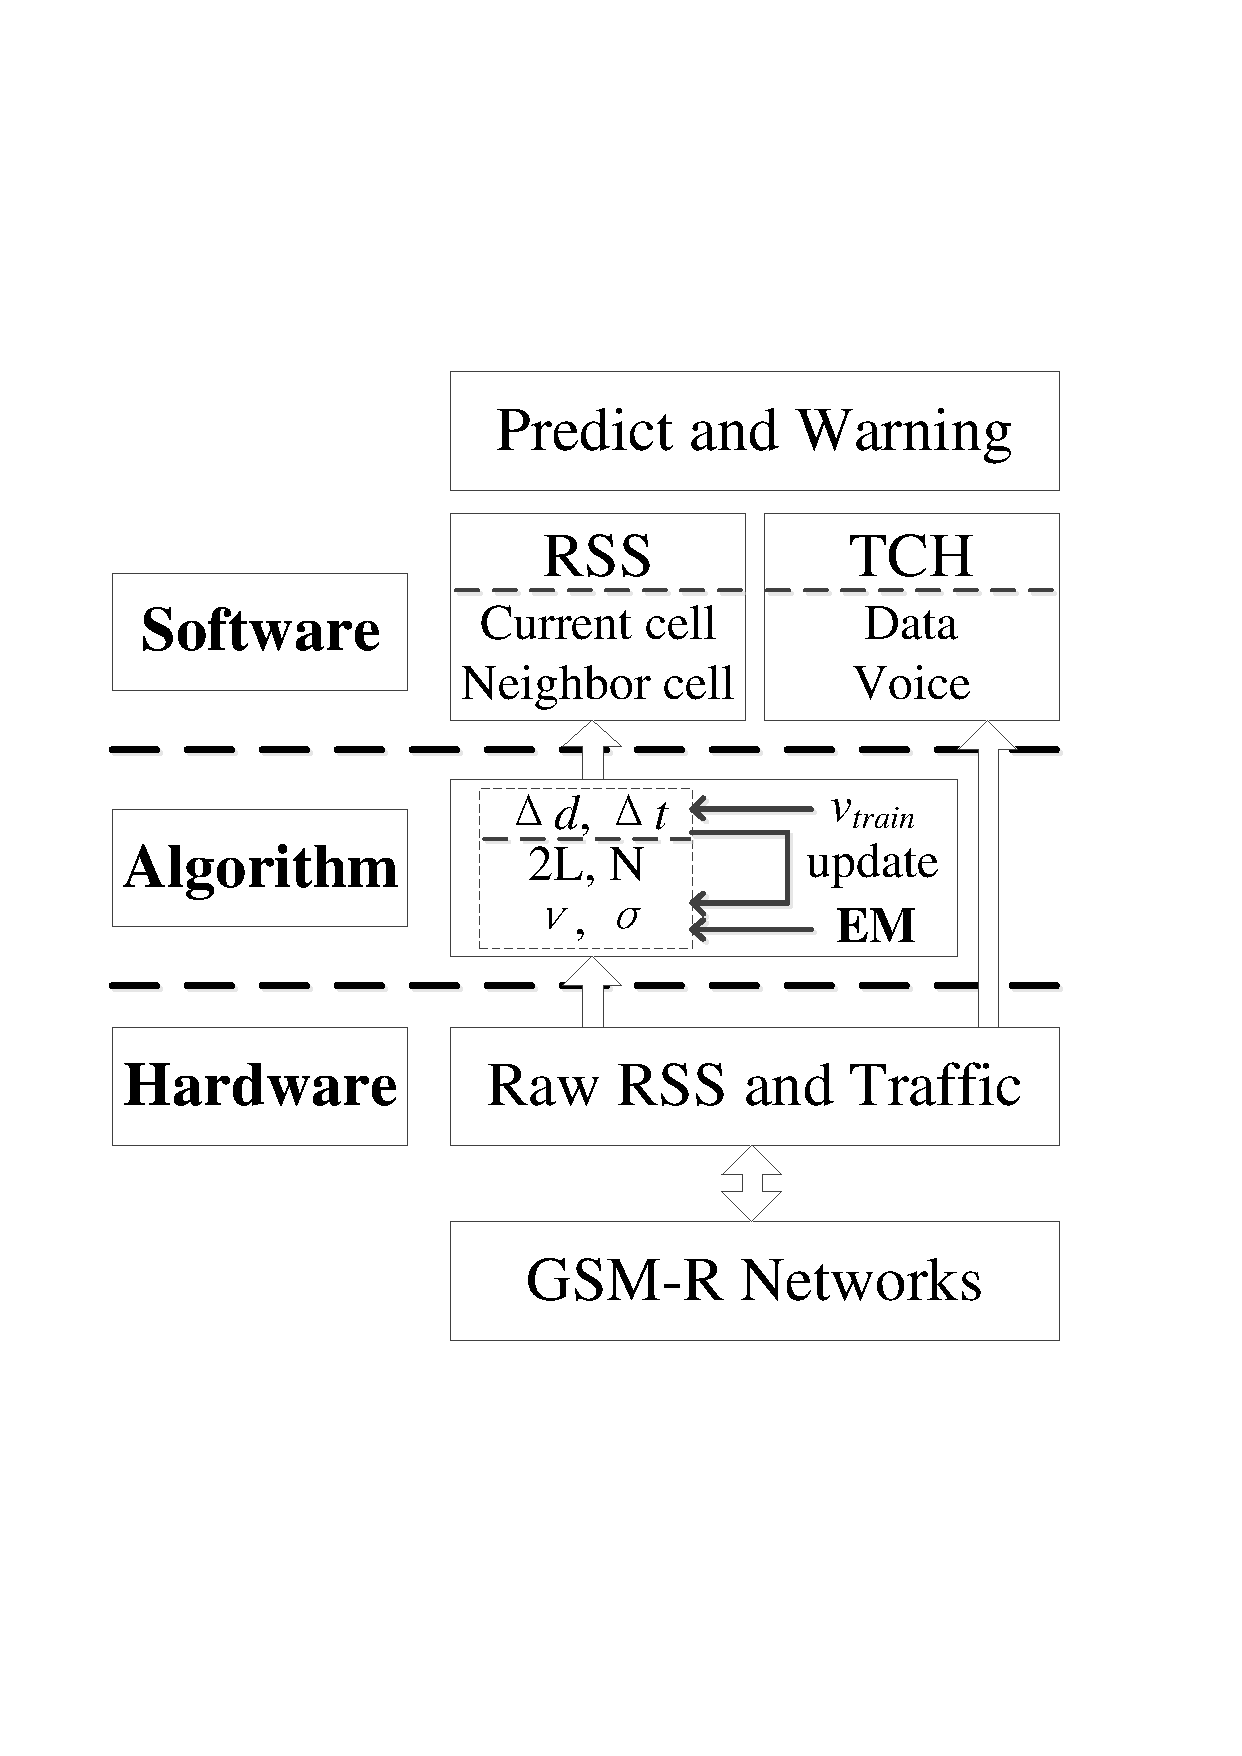
\includegraphics[width=4in]{chap2/umframework.pdf}
\bicaption[fig:umframework]{信道状态估计算法与实现}{信道状态估计算法与实现}{Fig}{Estimation framework and algorithm implementation}
\end{figure}

\subsection{基本功能}
\label{sec:function}

GSM-R网络空中接口测试系统的基本功能如图 \ref{fig:umsoftwarefunc} 所示,主要完成网络通信质量的测试、处理、预测、显示与预警。

\begin{figure}[!htp]
%\onelinecaptionsfalse
\centering
    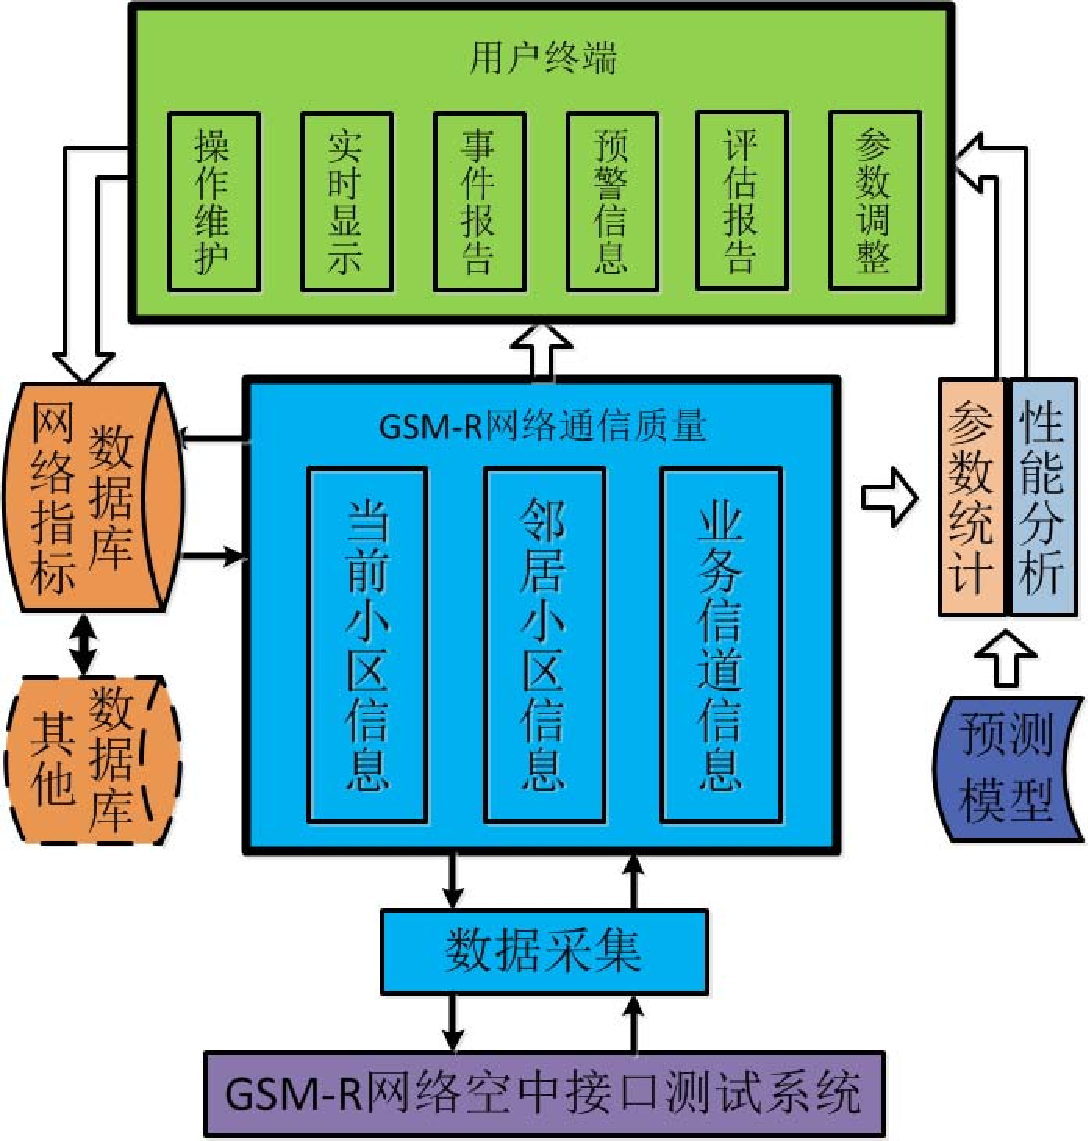
\includegraphics[width=4in]{chap2/function.pdf}
\bicaption[fig:umsoftwarefunc]{GSM-R网络空中接口测试系统软件结构}{GSM-R网络空中接口测试系统软件结构}{Fig}{Software architecture of Um interface monitoring system for GSM-R networks}
\end{figure}

测试系统在硬件配置完成后,测试软件首先对GSM-R网络空中接口传输的信息进行解析,得到网络当前时刻与位置的通信质量信息,并根据GSM-R网络当前小区信息得到网络当前广播控制信道、语音业务信道和数据域业务信道质量信息,并给出小区切换和信道切换的分布图,同时绘制当前服务小区广播控制信道的接收信号强度和邻居小区广播控制信道接收信号质量的曲线轨迹,利用当前测试数据与历史数据,结合预测模型对网络的无线传播进行预测,在当前网络通信质量低于系统要求时给出警告信息,结合地理信息和基站信息,给出测试报告并对GSM-R网络性能进行整体评估。
\begin{itemize}
  \item 当前小区信息:显示移动台当前所在小区基本信息,包括小区编号、信道编号、接收信号强度、基站识别码、功率等级和小区重选系数等信息。
  \item 邻居小区信息:显示接收信号强度最好的三个到六个邻居小区的信息,包括信道编号、接收信号强度、基站识别码和小区重选系数等。
  \item 业务信道信息:显示当前业务信道基本信息,包括信道编号、时隙分配、时间提前量、功率大小、接收信号强度、接收信号质量和信道模式等。
  \item 曲线绘制:实时记录当前小区及邻居小区的接收信号强度信息,并能够调取历史数据和数据库中的数据,进行场景重现。
  \item 历史数据:导入或导出历史数据,实现对任意时刻的通信情况进行分析,为GSM-R网络的优化提供数据支持。
\end{itemize}

\begin{figure}[!htp]
%\onelinecaptionsfalse
\centering
    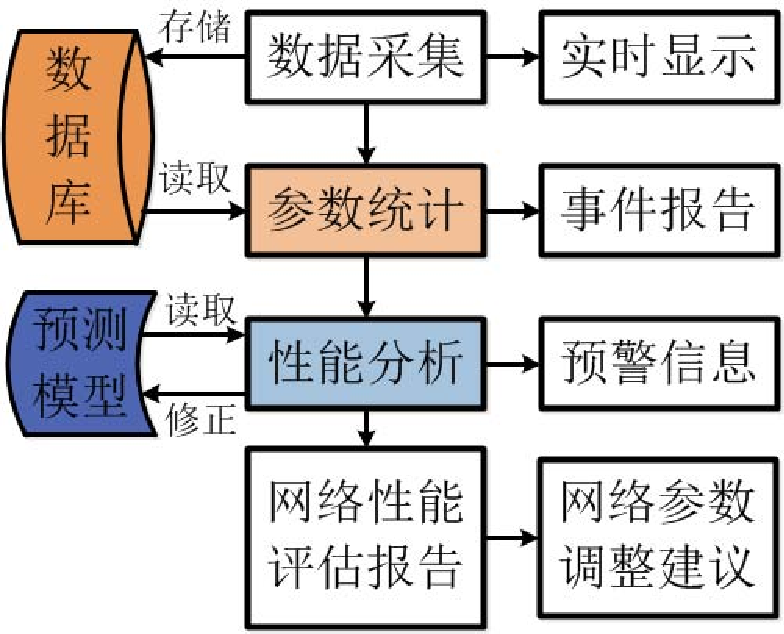
\includegraphics[width=3in]{chap2/dataprocess.pdf}
\bicaption[fig:umprocess]{GSM-R网络空中接口测试系统数据处理}{GSM-R网络空中接口测试系统数据处理}{Fig}{Data processing of Um interface monitoring system for GSM-R networks}
\end{figure}


\section{性能评估}
\label{chap:evaluation_phy}

本节主要介绍动态测试算法的实验分析与性能评估,通过GSM-R网络空中接口测试系统,由高速列车上的移动终端在京沪高速铁路沿线进行接收信号强度信息采集,如图 \ref{fig:platform} 所示。

\begin{figure}[!htp]
\centering
\subfigure[硬件平台]{
    \label{fig:hardware}
    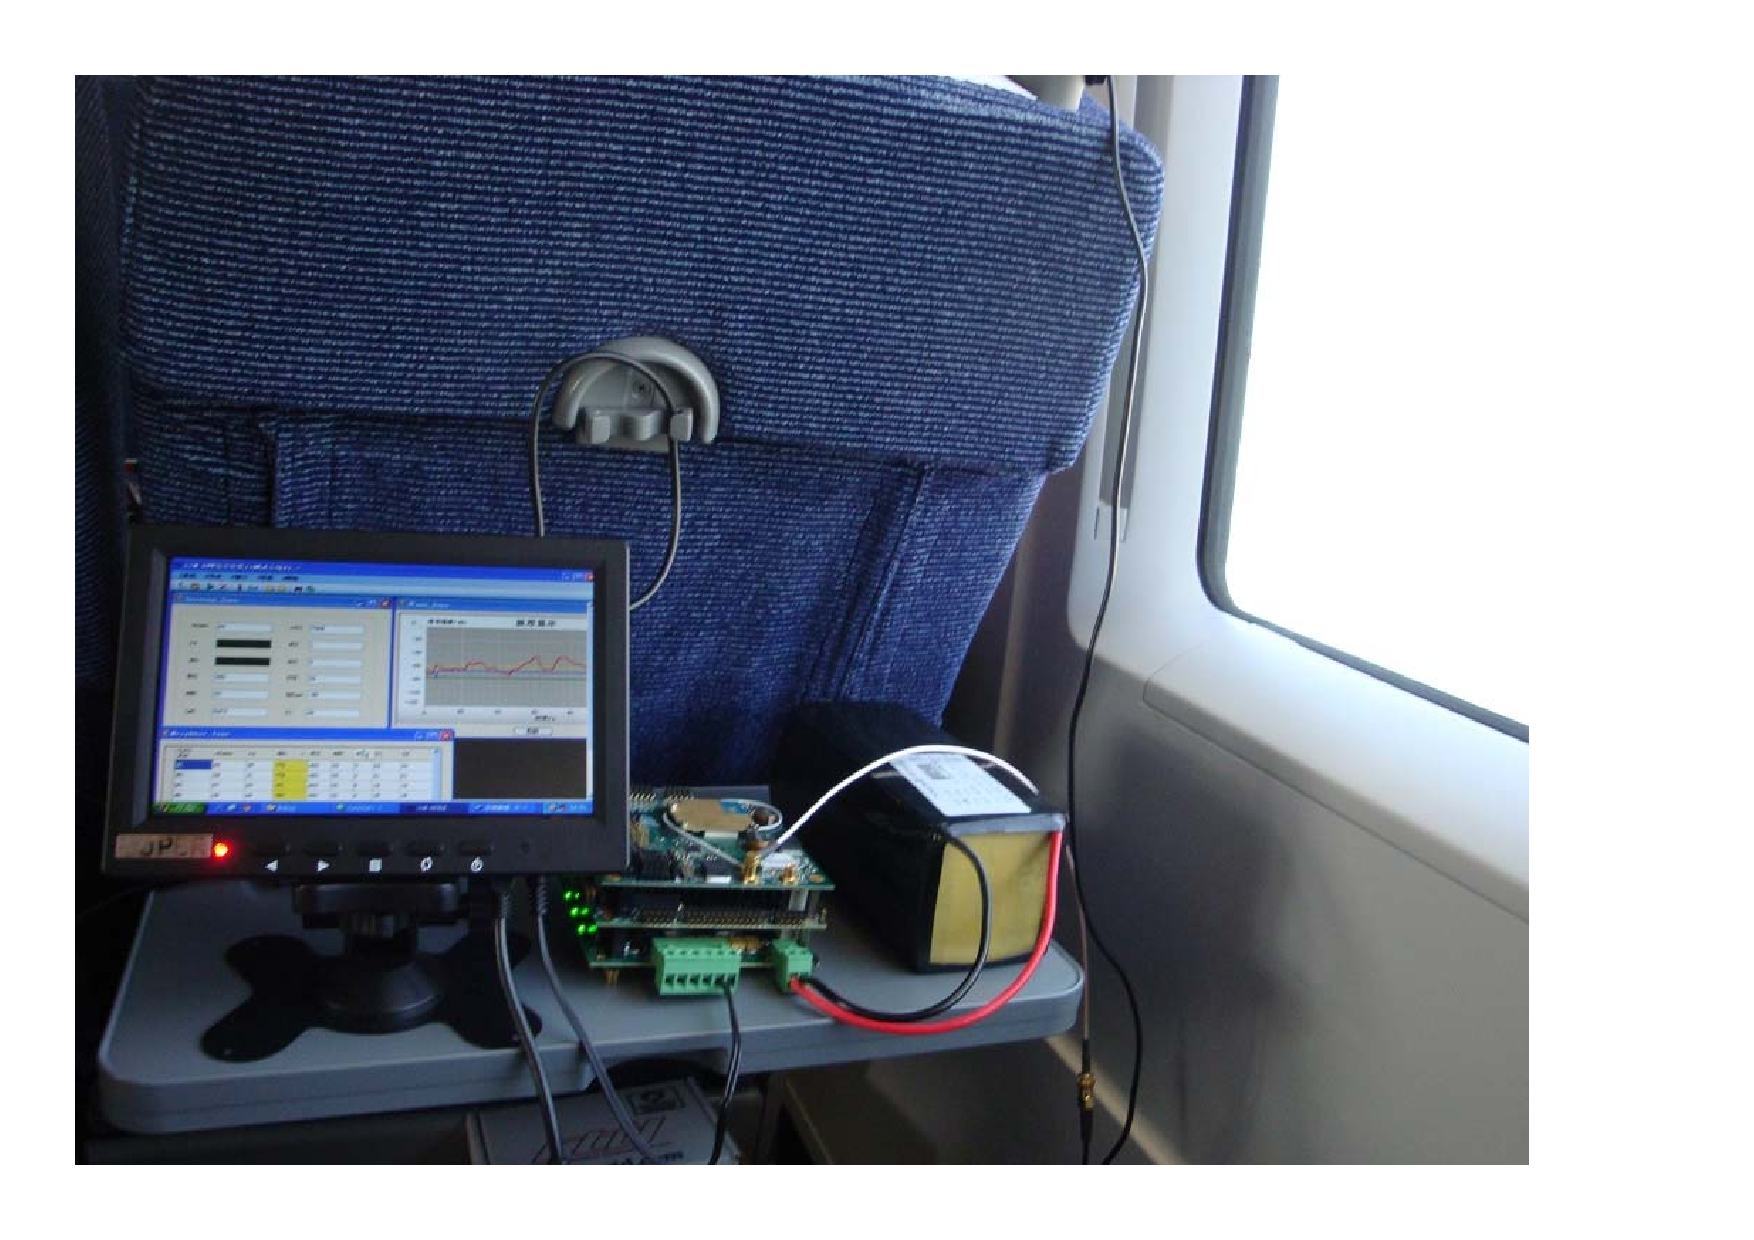
\includegraphics[width=2.5in]{chap2/platform.pdf}}
    \hspace{1cm}
\subfigure[软件平台]{
    \label{fig:software}
    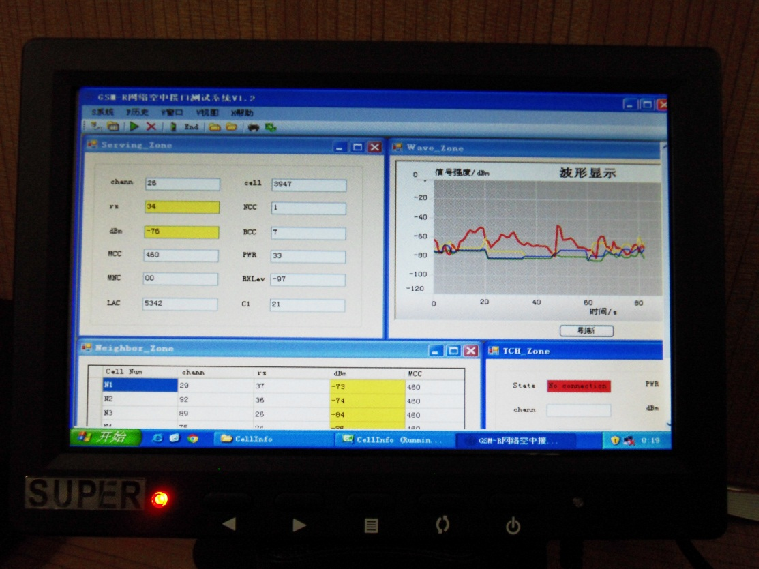
\includegraphics[width=2.5in]{chap2/softwareinterface.pdf}}
\bicaption[fig:platform]{GSM-R网络空中接口测试系统}{GSM-R网络空中接口测试系统}{Fig}{Um Interface Monitoring System for GSM-R Networks}
\end{figure}

实验测试结果以XML格式进行存储与处理,如图 \ref{fig:xml} 所示为京沪高铁GSM-R网络接收信号强度信息。动态估计算法的测试结果如表 \ref{tab:summary} 所示,包括不同无线传播环境下的莱斯衰落参数与采样参数,其中无线传播类型由莱斯衰落参数$K$表示:当$K=0$时表示没有直射路径信号,此时莱斯衰落退化为瑞利衰落;当$K$逐步增加表示无线传播环境逐渐平坦。

\begin{figure}[!htp]
\centering
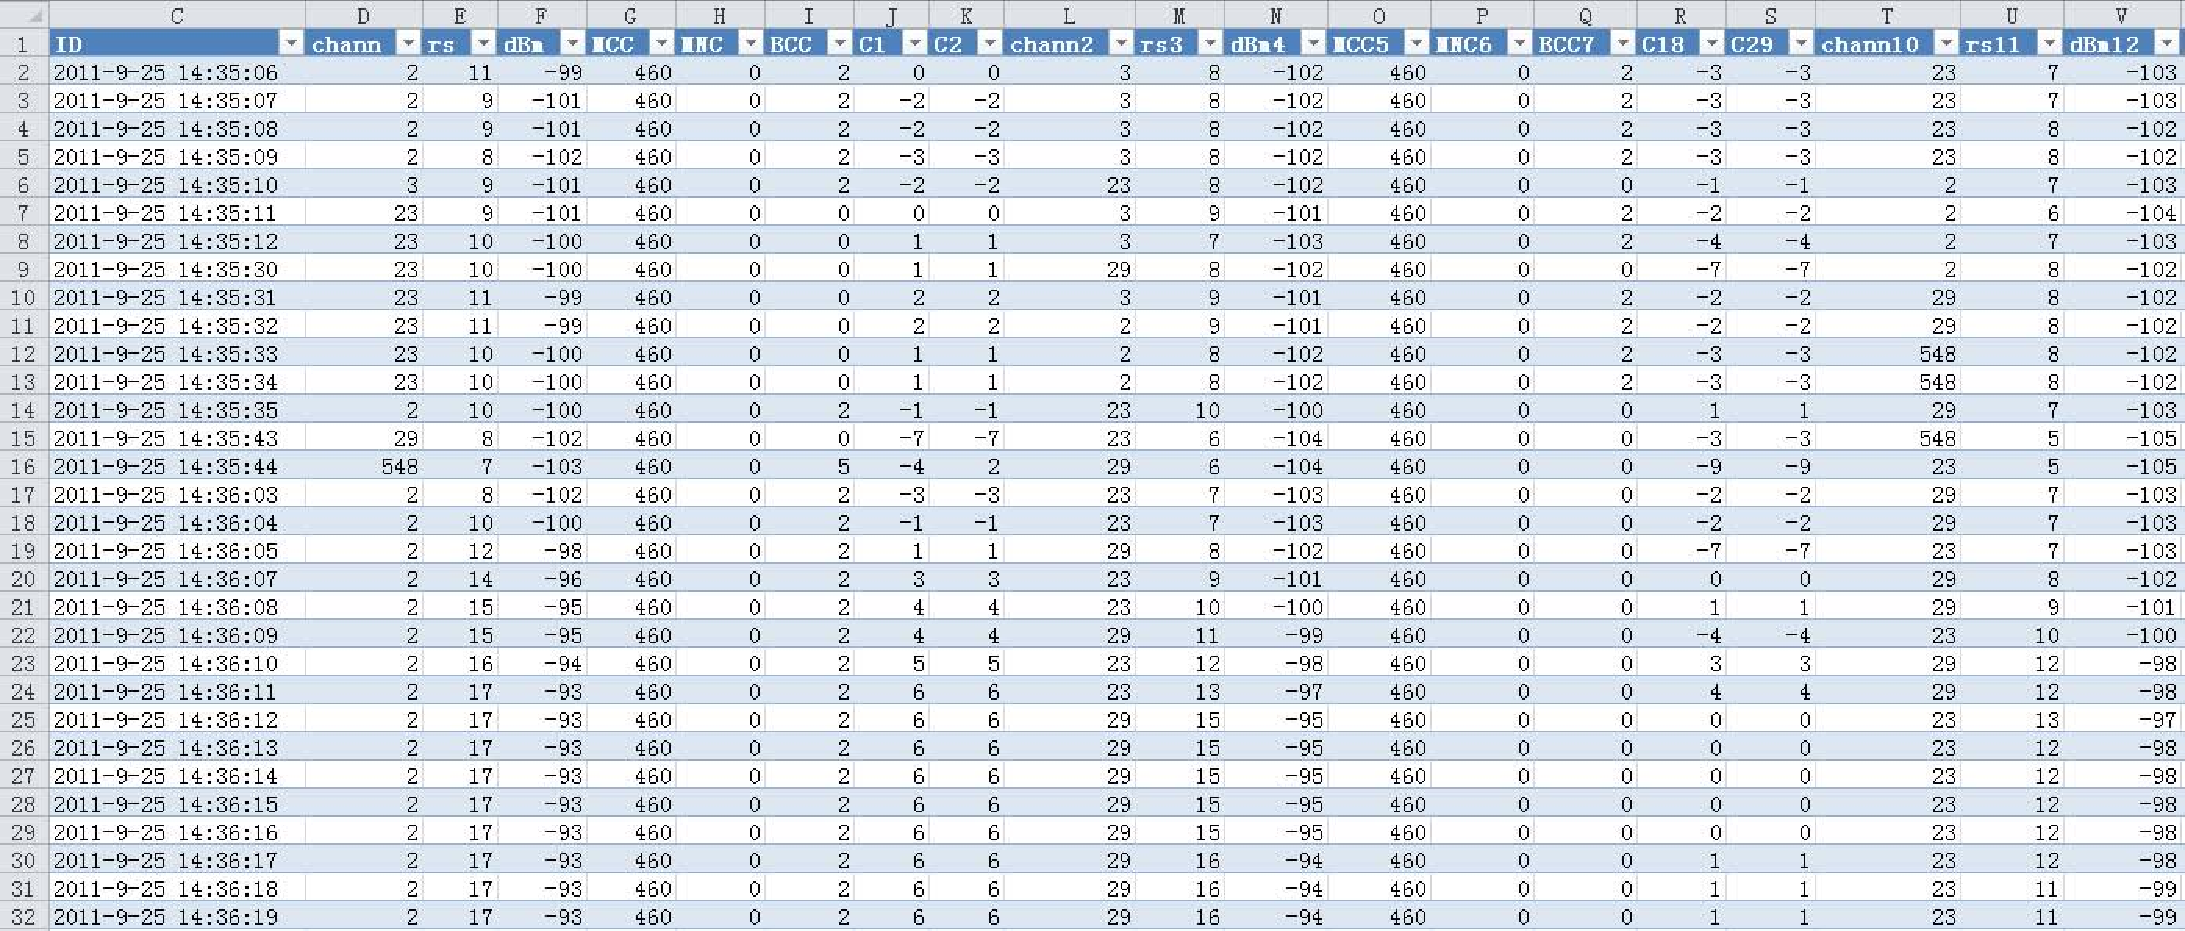
\includegraphics[width=1\textwidth]{chap2/xml.pdf}
\bicaption[fig:xml]{信道状态测试结果}{信道状态测试结果}{Fig}{Measurement Results}
\end{figure}

从表 \ref{tab:summary} 中的数据可以看出,在莱斯因子$K = 0$时,统计区间为$2L = 40\lambda$,采样间隔为$\Delta d = 0.5\lambda$;随着莱斯因子$K$的增大,无线传播环境逐渐平坦,导致直射路径功率比例增加,统计区间与采样间隔逐渐降低;当$\nu \geq 8$时所需的采样点数$N \leq 10$,即在不同统计区间内只需做$N \leq 10$次采样,便可以保证本地均值的准确性,同时在$K$值逐渐增大过程中,统计区间相应增大,且不需要做频繁的数据采集,采样间隔在$1m$左右。

\begin{table}[!htp]
\renewcommand{\arraystretch}{1}
\bicaption[tab:summary]{信道状态估计结果总结}{信道状态估计结果总结}{Table}{Summary of Experiment Results of Channel State Estimation}
\centering
\begin{threeparttable}[b]
\begin{tabular}{c|c|c|c|c|c|c|c|c|c|c}
%\toprule
\hline
%\cline{1-11}
\multicolumn{1}{c|}{\multirow{3}{*}{Terrain}} & \multicolumn{1}{c|}{\multirow{3}{*}{$K$(dB)}} & \multicolumn{1}{c|}{\multirow{3}{*}{$\nu$}} & \multicolumn{1}{c|}{\multirow{3}{*}{$\sigma$}} & \multicolumn{1}{c|}{\multirow{3}{*}{$2L/\lambda$}} & \multicolumn{1}{c|}{\multirow{3}{*}{$N$}} & \multicolumn{1}{c|}{\multirow{3}{*}{$\Delta d/\lambda$}} & \multicolumn{1}{c|}{\multirow{3}{*}{$\Delta d$(m)}} & \multicolumn{3}{c}{$v_{train}$(km/h)}\\
\cline{9-11}
\multicolumn{1}{c|}{} & \multicolumn{1}{c|}{} & \multicolumn{1}{c|}{} & \multicolumn{1}{c|}{} & \multicolumn{1}{c|}{} & \multicolumn{1}{c|}{} & \multicolumn{1}{c|}{} & \multicolumn{1}{c|}{} & 200 & 250 & 300\\
\cline{9-11}
\multicolumn{1}{c|}{}& \multicolumn{1}{c|}{} & \multicolumn{1}{c|}{} & \multicolumn{1}{c|}{} & \multicolumn{1}{c|}{} & \multicolumn{1}{c|}{} & \multicolumn{1}{c|}{} & \multicolumn{1}{c|}{} & \multicolumn{3}{c}{$\Delta t$(ms)}\\
%\midrule[5pt]
%\hline
%\hline
\cline{1-11}
NLOS\tnote{*}  &  0 &    - & - & 40 & 36 &  1.1 & 0.367 &  2.20 &  1.76 &  1.47\\
\hline
Dense &  0 &   0 & 1 & 55 & 15 &  3.7 & 1.222 &  7.33 &  5.86 &  4.89\\
      &  2 &   4 & 2 & 18 & 12 &  1.5 & 0.500 &  3.00 &  2.40 &  2.00\\
      &  4 & 5.6 & 2 &  9 &  9 &  1.0 & 0.333 &  2.00 &  1.60 &  1.33\\
      &  6 &   6 & 3 & 20 &  7 &  2.9 & 0.967 &  5.80 &  4.64 &  3.87\\
      &  8 &  12 & 3 &  8 &  1 &  8.0 & 2.667 & 16.00 & 12.80 & 10.67\\
Open  & 10 &  18 & 4 & 12 &  1 & 12.0 & 4.000 & 24.00 & 19.20 & 16.00\\
%\bottomrule[10pt]
\hline
%\cline{1-11}
\end{tabular}
\begin{tablenotes}
\item[*] \small 在瑞利衰落信道情况下,通过Lee氏采样算法的计算结果
\end{tablenotes}
\end{threeparttable}
\end{table}

\begin{figure}[!htp]
\centering
    \subfigure[接收信号强度与大尺度衰落]{
    \label{fig:input}
    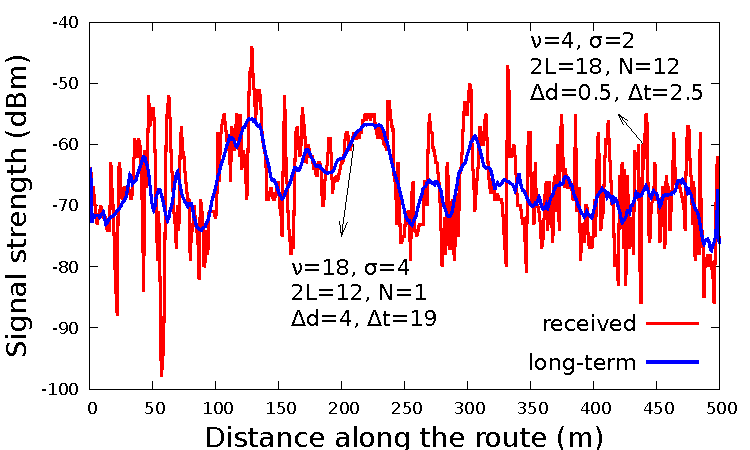
\includegraphics[width=4.5in]{chap2/em.pdf}}
\hspace{1in}
\centering
    \subfigure[小尺度衰落]{
    \label{fig:output}
    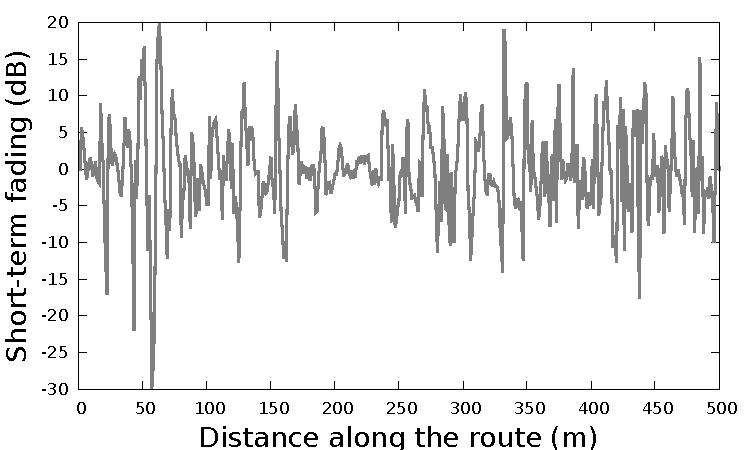
\includegraphics[width=4.5in]{chap2/short.pdf}}
\bicaption[fig:strength]{接收信号强度与信号衰落}{接收信号强度与信号衰落}{Fig}{Received signal strength and signal fading}
\end{figure}

对于运行于900MHz的GSM-R网络而言,Lee氏采样算法的采样间隔为$36cm$,工程应用中采用每隔$4cm$的采样方式,在相同的测试精度的前提下,即保证归一化误差为1dB,动态采样算法能够实现测试误差的显著降低,从而在完成通信性能测试的同时保证网络的正常通信。

通过动态测试算法获得的接收信号强度信息如图 \ref{fig:strength} 所示,大尺度和小尺度衰落经过动态测试算法能够有效区分,从而能够进行分别分析与处理。大尺度衰落通过最大似然估计或最小均方差估计,实现无线传播预测或模型修正;小尺度衰落对于无线网络的切换算法、功率控制及频谱分配等具有重要影响,例如切换算法中切换门限的选择与设置。

\section{本章小结}
\label{sec:conclusion2}

本章讨论了在莱斯衰落环境下,GSM-R网络接收信号强度的动态采样算法,解决高速移动性及传播环境复杂性对信道采样的不利影响。该算法通过采样数据结合衰落参数历史值,对当前衰落参数进行估计,确定不同衰落参数条件下的统计区间与采样点数。在城区、山地、丘陵等密集区域,由于多径衰落现象加重,且直射路径功率所占比例较低,需要进行较为频繁的采样与统计,确保统计区间$2L \leq 20m$,采样间隔$\Delta d \leq 0.3m$;在平原、高架桥等开阔区域,移动台接收功率较大,且一般存在较大比例的直射路径功率,在同样的统计区间内只需做较少的采样,保证统计区间$2L \leq 50m$,采样间隔$\Delta d \leq 1.5m$,便可以满足本地均值的准确性要求。对应列车运行速度在$300km/h$ 时,采样时间间隔为$2.0ms$到$18.0ms$ 时,才能够保证测量数据的可靠性。在实际工程应用中的GSM-R 网络无线覆盖测量,一般采用采样间隔$\Delta d = 4cm$、统计区间$10m \leq 2L \leq 100m$ 的方法,参照本章关于莱斯衰落信道下采样算法的推导,可以在高铁线路中的开阔区域适当提高采样间隔,从而在确保数据可靠性的同时降低测量开销;另一方面针对GPS测距触发方式的测量方法,利用高速铁路列车运行速度相对固定的特点,结合列车运行速度、当前采样数据及衰落参数历史数据,采用时间触发的方式进行采样间隔与统计区间的确定。

\nocite{Akhoondzadeh2007modifi,andersen1995propagation,bjornson2010framework,gopal2009power,itoh2002performance}
\nocite{sijbers1998maximum,zhang1996analysis,zhu2005performance,mousa2010estimation}
\nocite{saleh1987statistical}
\nocite{goldsmith1994error}
\nocite{aja2008restoration}
\nocite{saleh1987statistical}
\nocite{sijbers1998maximum}\nocite{devore2000atr}\nocite{mousa2010estimation}
